%%%%%%%%%%%%%%%%%%%%%%%%%%%%%%%%%%%%%
%% Supporting Information
%% (Optional)
%%%%%%%%%%%%%%%%%%%%%%%%%%%%%%%%%%%%%
% OVERVIEW
%
% Please note that all supporting information will be peer reviewed with your manuscript.
% In general, the purpose of the supporting information is to enable
% authors to provide and archive auxiliary information such as data
% tables, method information, figures, video, or computer software,
% in digital formats so that other scientists can use it.

% The key criteria are that the data:
% 1. supplement the main scientific conclusions of the paper but are not essential to the conclusions (with the exception of
%    including data so the experiment can be reproducible);
% 2. are likely to be usable or used by other scientists working in the field;
% 3. are described with sufficient precision that other scientists can understand them, and
% 4. are not exe files.
%

% All Supporting text and figures should be included in this document.

% Data sets, large tables, movie files,
% and audio files should be uploaded separately, following AGU naming
% conventions. Include their captions in this document and list the
% file name with the caption. You will be prompted to upload these
% files on the Upload Files tab during the submission process, using
% file type “Supporting Information (SI)”

\documentclass[draft]{agujournal}
\graphicspath{{figures/}}

% \usepackage{amsmath}
% \usepackage{apacite}
% \usepackage[inline]{trackchanges}
\usepackage{float}
\usepackage{enumitem}
%\usepackage[font=normalsize]{caption}
% \bibliographystyle{agu08}
% \setcitestyle{authoryear,open={[},close={]}}

\usepackage{titlesec}
\titleformat{\section}{\normalfont\Large\bfseries}{S\thesection}{1em}{}
\titleformat{\subsection}{\normalfont\large\bfseries}{S\thesubsection}{1em}{}


%\renewcommand{\figurename}{Figure S}
%\renewcommand{\tablename}{Table S}

\renewcommand\thefigure{S\arabic{figure}}
\renewcommand\thetable{S\arabic{table}}

% Please type in the journal name: \journalname{<Journal Name>}
% ie,
\journalname{Journal of Geophysical Research}

%% Choose from this list of Journals:
%
% Journal of Geophysical Research
% JGR-Biogeosciences
% JGR-Earth Surface
% JGR-Planets
% JGR-Solid Earth
% JGR-Space Physics
% Global Biochemical Cycles
% Geophysical Research Letters
% Paleoceanography
% Radio Science
% Reviews of Geophysics
% Tectonics
% Space Weather
% Water Resource Research
% Geochemistry, Geophysics, Geosystems
% Journal of Advances in Modeling Earth Systems (JAMES)
% Earth's Future
% Earth and Space Science

\begin{document}

%% This command needs article title as argument to \supportinginfo{}:
\supportinginfo{What controls variations in aftershock productivity?}

\authors{Kelian Dascher-Cousineau \affil{1},
 Emily E. Brodsky \affil{1}, Thorne Lay \affil{1}
 Thomas H. W. Goebel \affil{2}}
 
\affiliation{1}{University of California Santa Cruz, Santa Cruz, California, USA.}
\affiliation{2}{University of Memphis, Memphis, Tennessee}

\large
\section*{Contents}
\begin{minipage}{.8\textwidth}

    \begin{enumerate}[label=\textbf{S\arabic*}]
    \item Critical examination of relative productivity\dotfill \pageref{sec:Critical}
    \begin{enumerate}[label*=\textbf{.\arabic*}]
    \setlength{\itemindent}{1.5em}
        \item Scaling effects\dotfill \pageref{sec:Critical}
        \item Catalog completeness\dotfill \pageref{sec:catalog}
        \item Alternative clustering method\dotfill \pageref{sec:alt}
        \item Background Seismicity\dotfill \pageref{sec:background}
    \end{enumerate}
    
    \item Relative productivity as a function of miscellaneous parameters \dotfill \pageref{sec:relative}
    \item{Additional Supporting Information (Files uploaded separately)}\dotfill \pageref{sec:additional}
    \begin{enumerate}[label*=\textbf{.\arabic*}]
    \setlength{\itemindent}{1.5em}
        \item Trained SVM  model\dotfill \pageref{sec:trained}
        \item Catalogued source attributes\dotfill \pageref{sec:source}
        \item Alternative clustering code\dotfill \pageref{sec:aftershock}
    \end{enumerate}
    \end{enumerate}
    
\end{minipage}

\section{Critical examination of relative productivity}
\label{sec:Critical}

In this section we  examine potential biases to relative productivity that may arise from our counting method, its parameterization and catalog artifacts.

\subsection{Scaling effects}\label{sec:scaling}

%(Figures \ref{fig:box_and_wiskers}) 
We first assess whether any biases are introduced by the definition of relative productivity as the number of aftershocks referenced to the number of aftershocks expected for a given magnitude. If the global trend with magnitude is incorrectly modelled, a systematic trend of relative productivity with magnitude would be observed. Figure \ref{fig:box_and_wiskers} shows that no such trend exists and thus definition of relative productivity appears reasonable.

%(Figures \ref{fig:prod_scaling}) 
Next, we examined whether there may be issues related to the definition of the scaling relationship we used in space windowing. Figure \ref{fig:prod_scaling} compares the measurement of relative productivity utilizing two different inferred scalings between rupture length and magnitude \citep{Brengman2019EarthquakeScalingDistributions,Wells1994}. We find that 79\% of sequences have the same aftershock counts regardless of the scaling used and that the excursions tend to be small.

%(Figures \ref{fig:caltech_sens2}-\ref{fig:caltech_sens2})
Using a the group of earthquakes with $M_W<7.5$ reveals more statistically significant subgroups for attributes which do not require finite fault inversion (Figure~\ref{fig:caltech_sens2}). Conversely, those attributes derived from finite fault inversion become less stable and, as a result, their relative productivity statistics are more varied (Figure~\ref{fig:caltech_sens1}). The attributes defining the largest and smallest relative productivity are the same in both cases.  Note that within for the set of smaller mainshocks, the median value of relative productivity can be censored, implying that the median mainshock of the subgroup had no measured aftershock.

\begin{figure}[H]
\centering
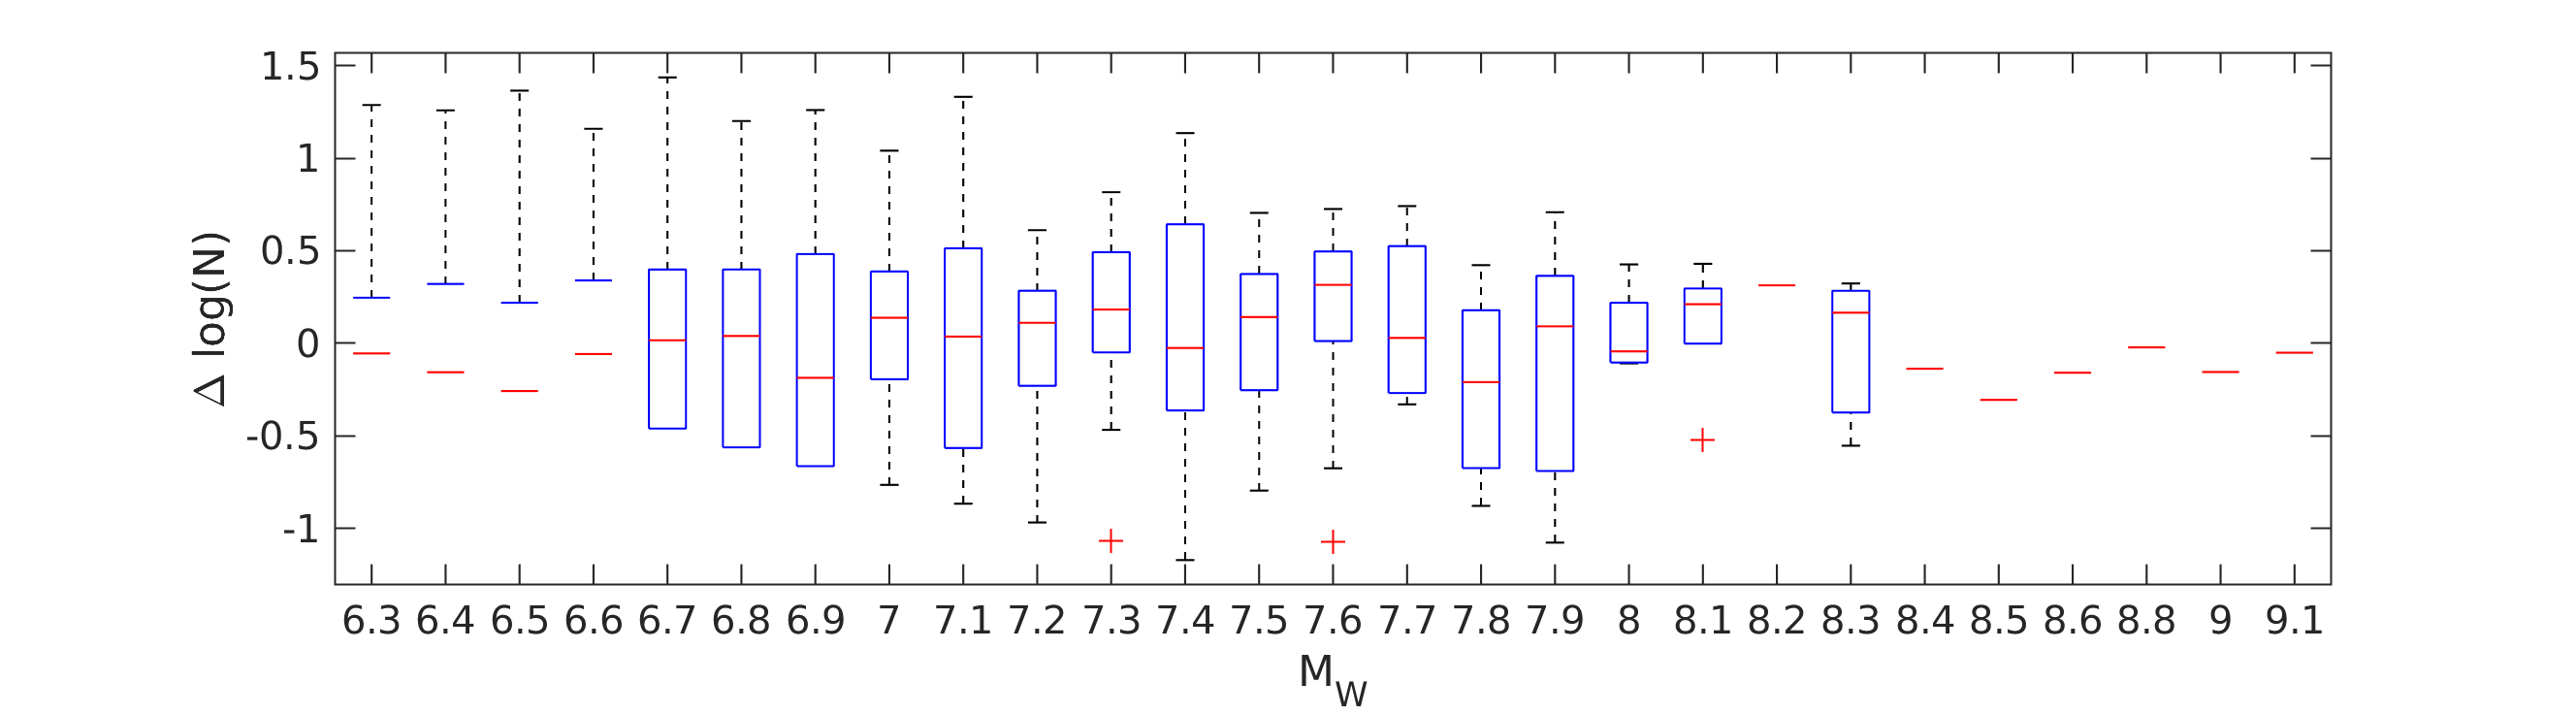
\includegraphics[width=\textwidth]{figures/box_and_wiskers.png}
\caption{Box and whiskers plot of relative productivity as a function of magnitude. Boxes outline the interquartile range. Whiskers outline the range of the data and +'s indicate outliers. Censoring, $\Delta\log(N) = -inf$, at the lower magnitudes ($M_W<6.7$) and limited data at highest magnitudes ($M_W>8.1$) prevent proper assessments of the interquartile range. Nonetheless, we do not observe a systematic decrease in variance that may introduce bias in subsequent analysis.}
\label{fig:box_and_wiskers}
\end{figure}

\begin{figure}[H]
\centering
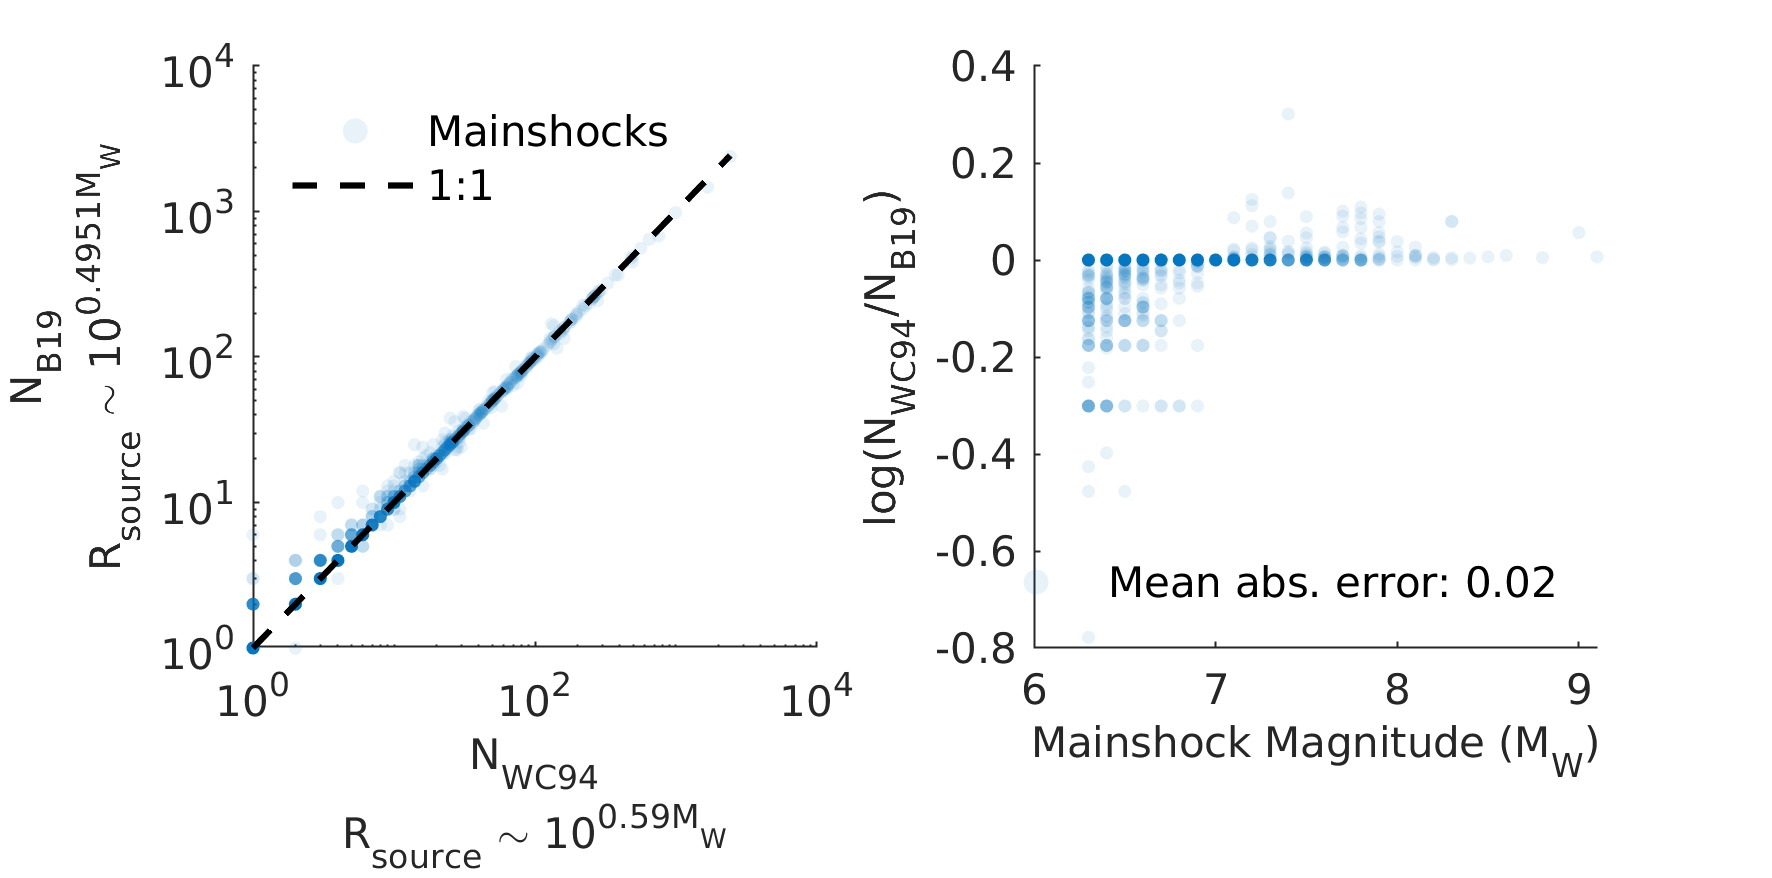
\includegraphics{figures/scaling_comparison.png}
\caption{Comparison between relative productivity statistic as obtained from two different scaling relationships: 1) WC94 following \citep{Wells1994} and 2) B19 following \citep{Brengman2019EarthquakeScalingDistributions}. Left: Direct comparison of inferred number of aftershocks. Right: Discrepancy in measurements as a function of mainshock magnitude. We find that 79\% of sequences have that exact same aftershock counts. Larger ruptures yield slightly smaller a aftershock counts the B19 scaling, whereas smaller ruptures have the converse relationship. Generally, the effect is subtle with a mean absolute error of 0.02. Note that the discrepancies, $log(N_{WC}/N_{B19})$, are directly equal to differences in measurements of relative productivity.}
\label{fig:prod_scaling}
\end{figure}

\begin{figure}[H]
\centering
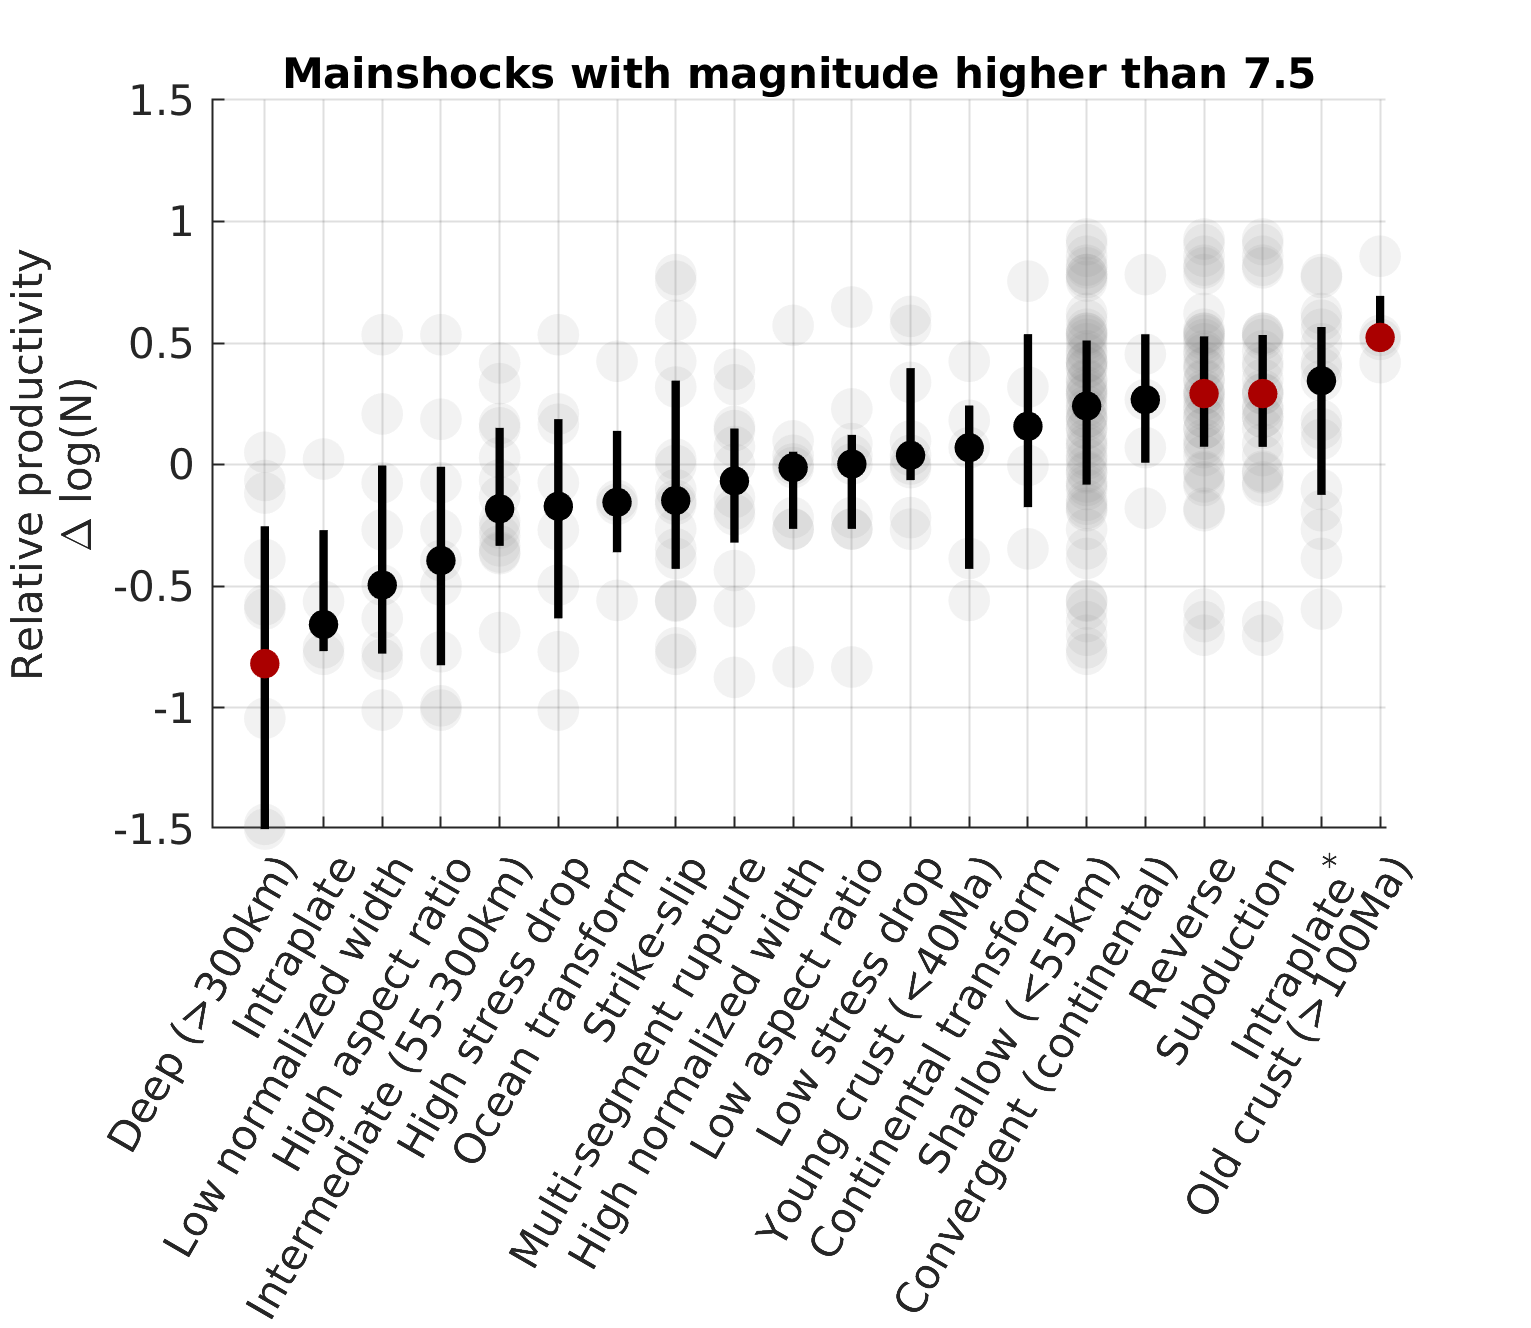
\includegraphics{figures/cal_tech_7plus.png}
\caption{Major results of this study presented for mainshocks with $M_W$ magnitude greater than 7.5. Attributes with red markers are more consistent with the hypothesis that they are sampled from a different continuous distribution than the overall population of earthquakes using a 2-sampled Kolmogorov-Smirnov test at a 5\% significance threshold.}
\label{fig:caltech_sens1}
\end{figure}

\begin{figure}[H]
\centering
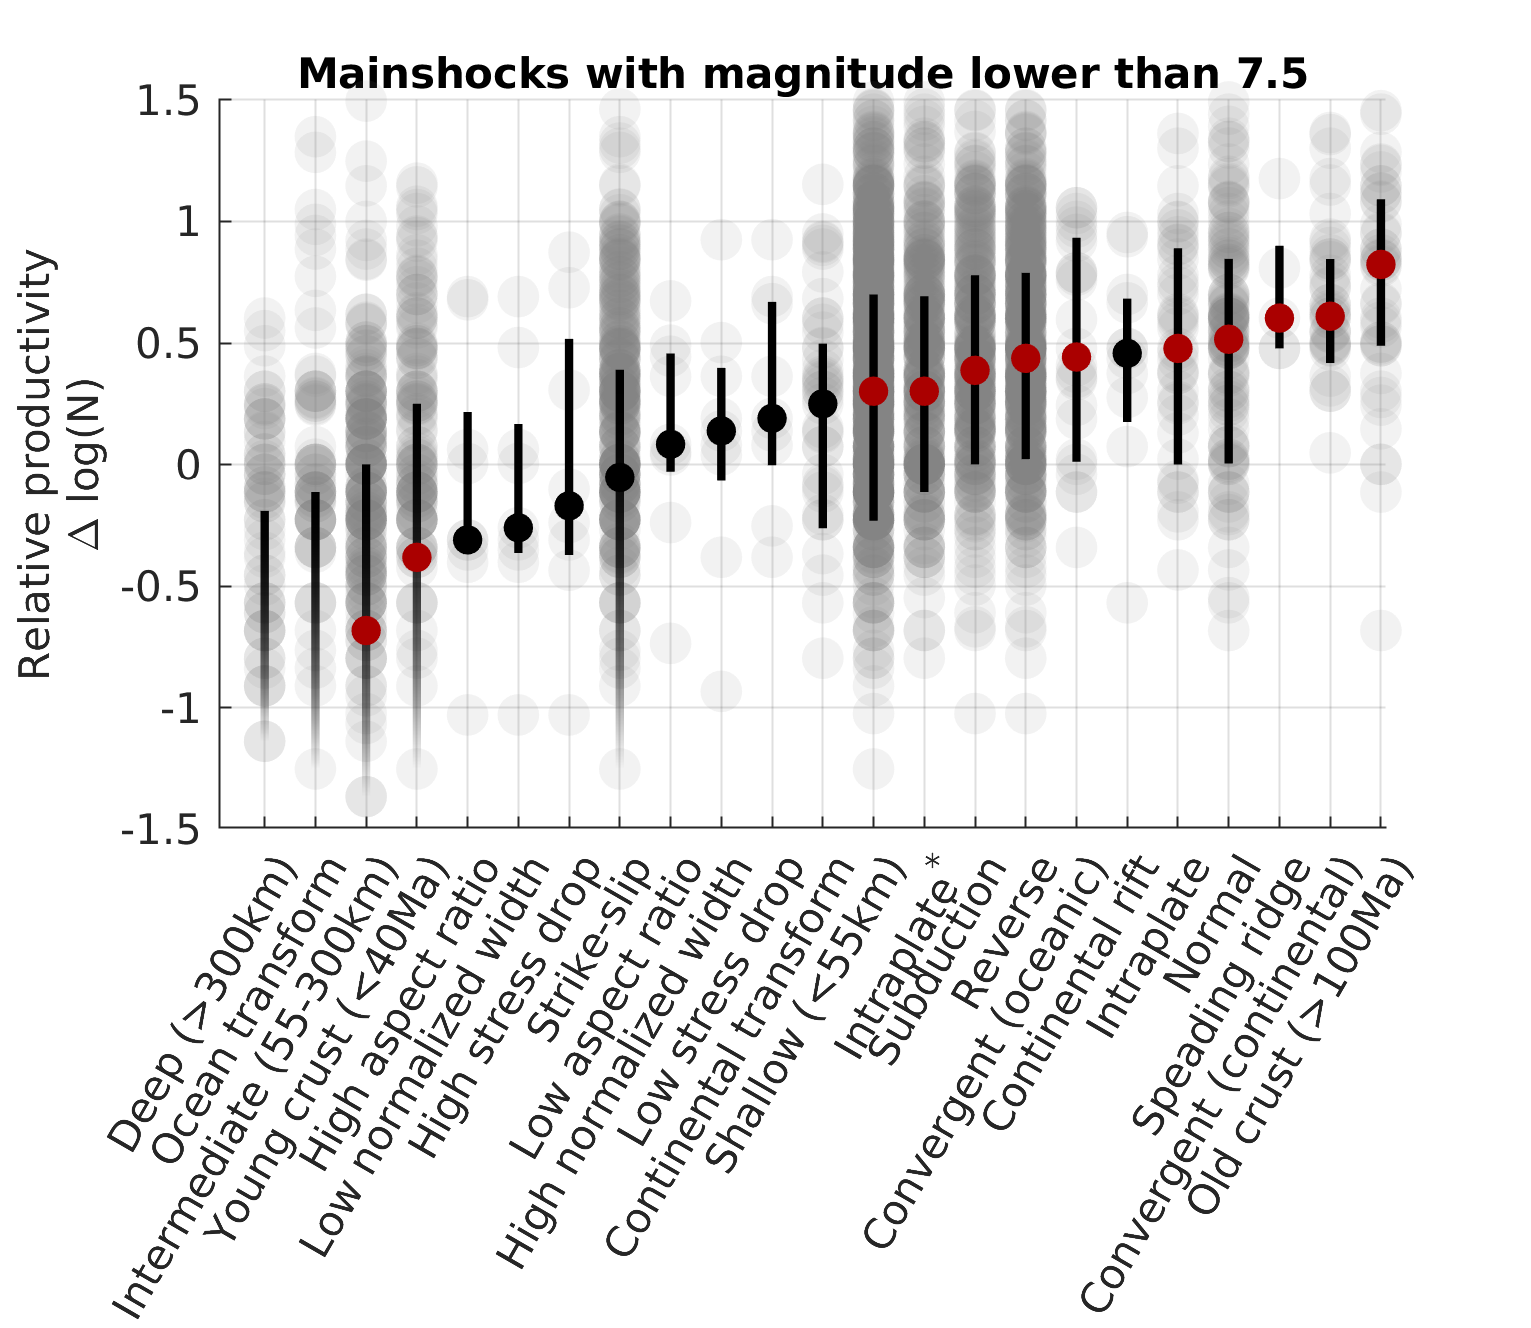
\includegraphics{figures/cal_tech_lt7.png}
\caption{Major results of this study presented for mainshocks with $M_W$ magnitude less than 7.5. Attributes with red markers are consistent with the hypothesis that they are sampled from a different continuous distribution than the overall population of earthquakes using a 2-sample Kolmogorov-Smirnov test at a 5\% threshold.}
\label{fig:caltech_sens2}
\end{figure}
%%%%%%%%%%%%%%%%%%%%%%%%%%%%%%%%%%%%%%%%%%%%%%%%%%%%%%%%%%%%%%%%%%%%%%%
\newpage
\subsection{Catalog completeness}\label{sec:catalog}
%(Figures \ref{fig:fms_prod}-\ref{fig:caltech}) 
We test the robustness of our primary findings by testing their validity with a more conservative magnitude of completeness of $M_w5$ instead of $M_w4.5$ as done in the main text. In these results, there are fewer aftershocks detected and statistical significance is therefore decreased while the chance of  inclusion of any background events in the counts is lowered because of the reduced rate for the larger magnitude cut-off, but the results do not violate any of the major findings of the main text.  We reproduce Figures~1--11 of the main text with the alternative completeness in Figures \ref{fig:fms_prod}--\ref{fig:caltech}, which preserve the same order as the main text. 

\begin{figure}[H]
\centering
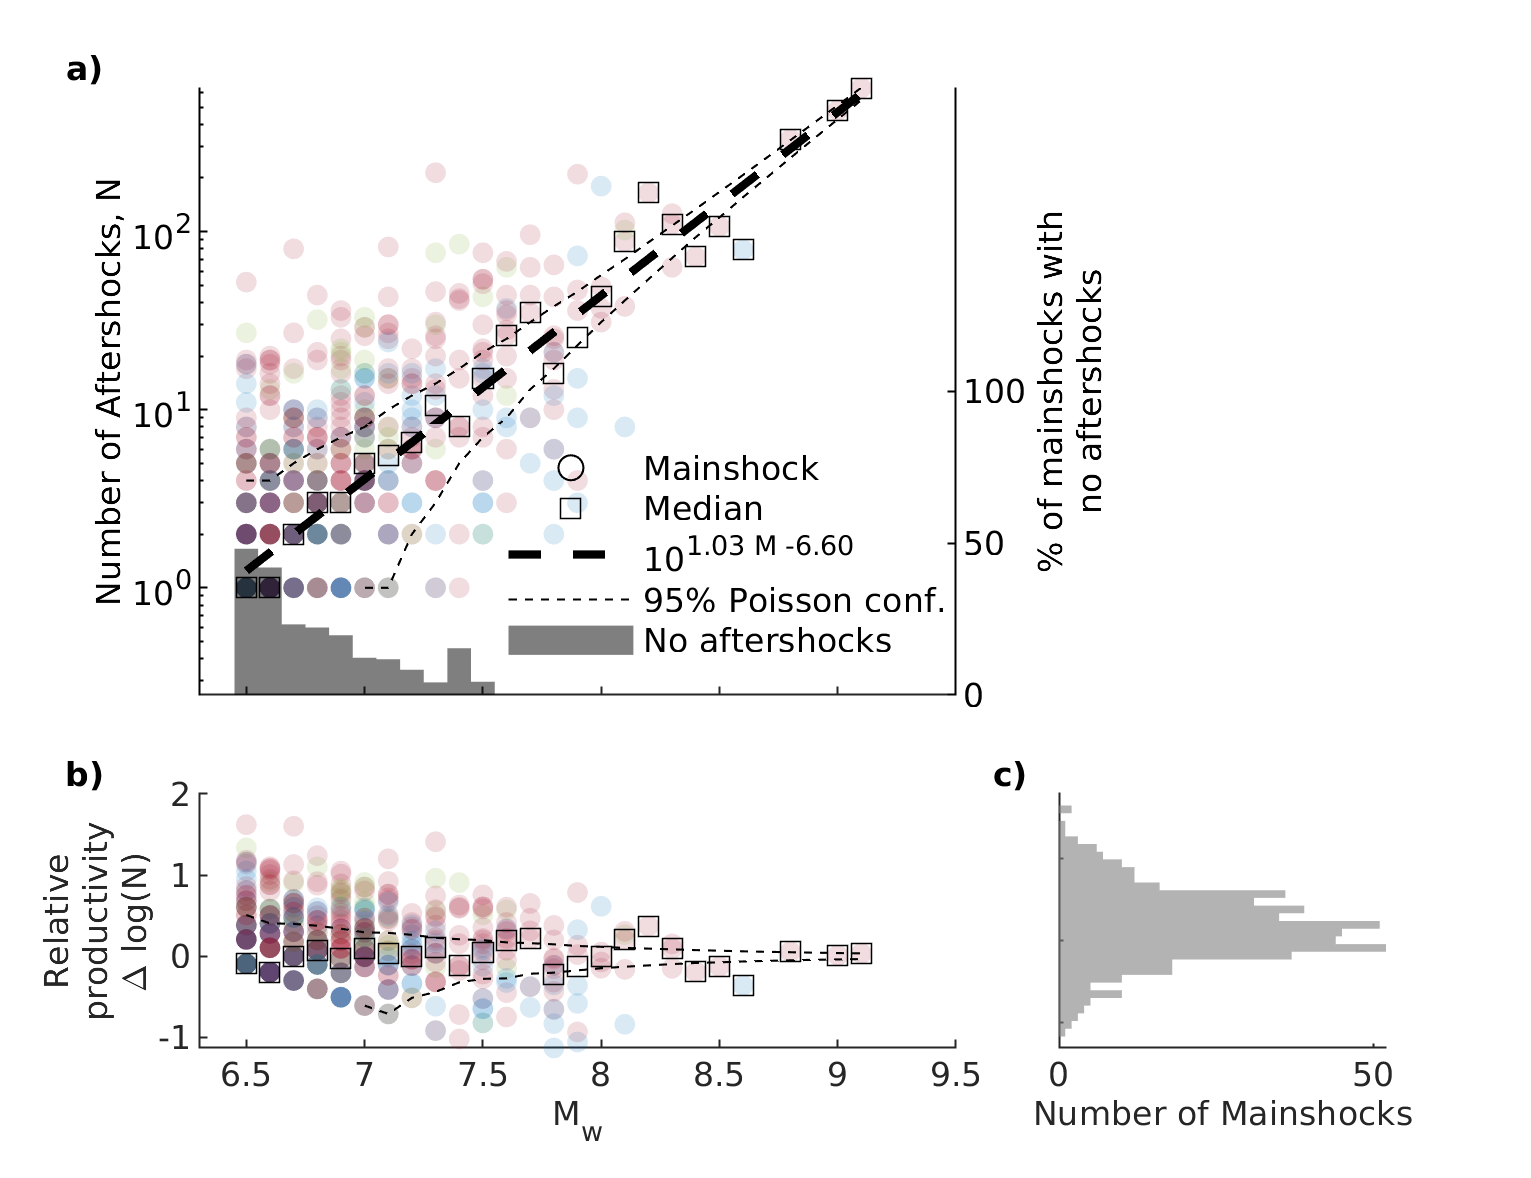
\includegraphics{figures/prod_law_mw5.png}
\caption{The number of aftershocks of $M_W\ge5$ within three source dimensions and 60 days as a function of mainshock magnitude identified in the global ISC and NEIC catalogs from 1990 to 2019. Colors indicate faulting style of the mainshock; blue, green and red points correspond to earthquake sequences for which the mainshock was respectively strike-slip, normal or reverse. The global productivity law (dashed line) is fit using a least squares regression through the median log-number of aftershocks for each 0.1 magnitude bin (black squares). The median number includes mainshocks with no aftershocks which are not shown on the plot. Note the individual earthquake sequences (circles) exhibit significant scatter around the productivity law. b) Relative productivity as a function of mainshock magnitude. The relative productivity distribution does not show events with no aftershocks and thus the lower left corner of the plot is underpopulated. c) Histogram of the relative productivity of mainshocks considered in this study.
}
\label{fig:fms_prod}
\end{figure}

\begin{figure}[H]
\centering
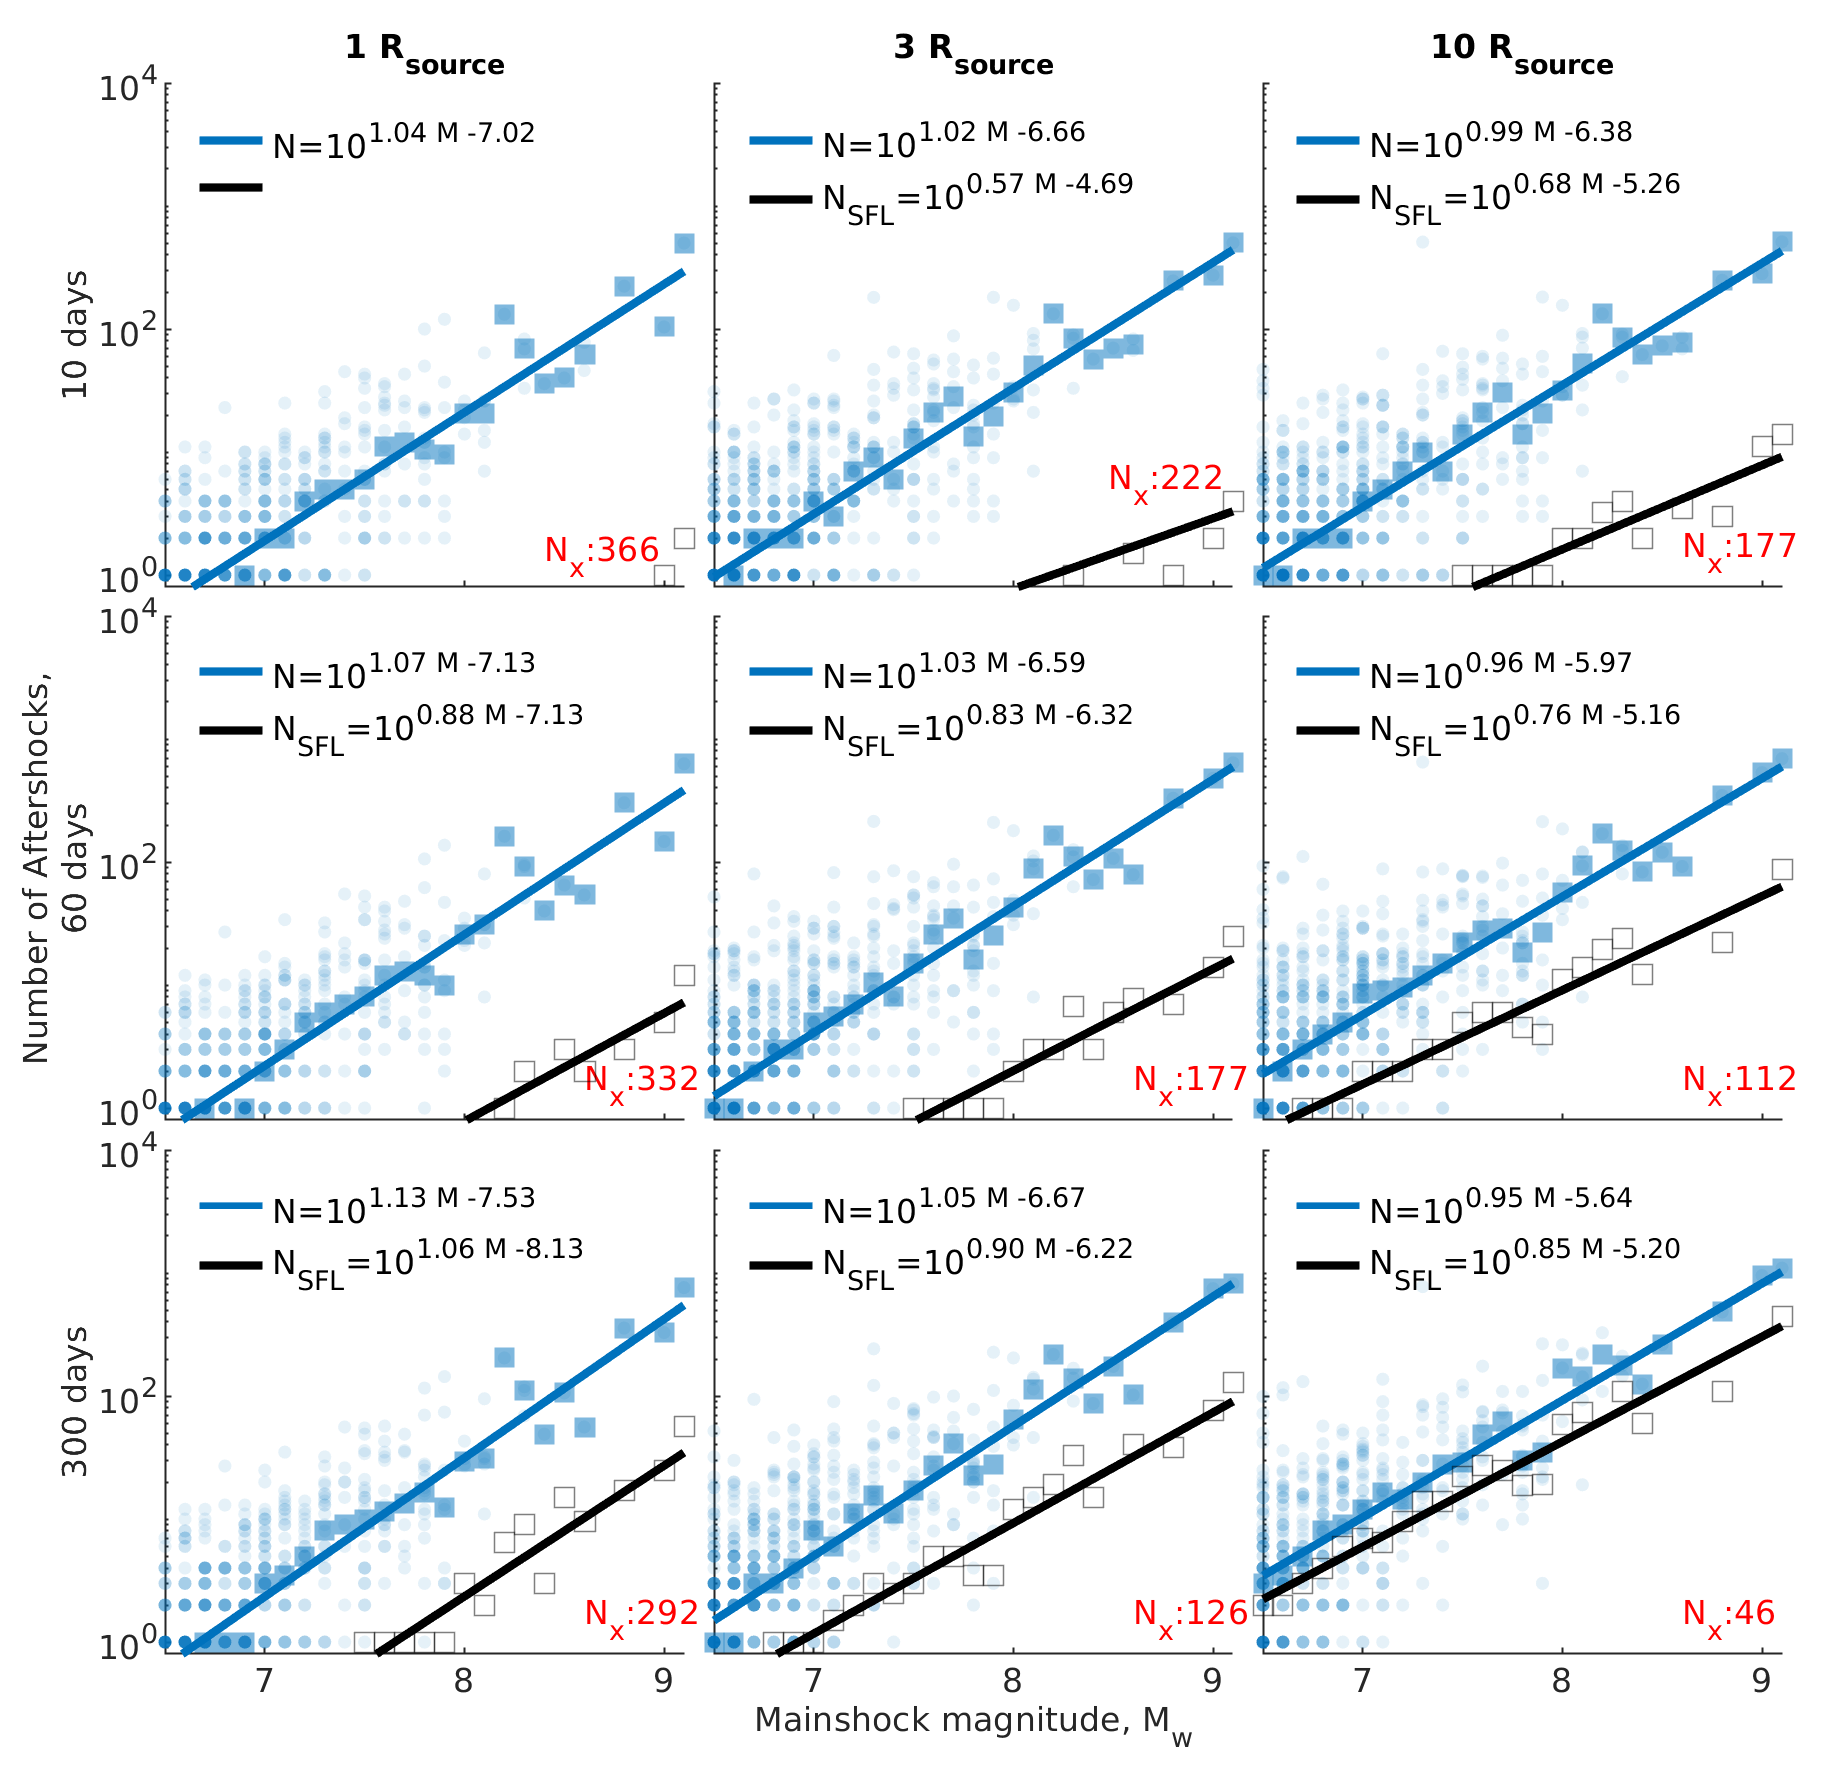
\includegraphics[width=\linewidth]{figures/sensitivity_mw5.png}
\caption{Sensitivity analysis of space-time windows. Time windows of 10, 60, and 100 days and spherical space with radii of 1, 3, and 10 source dimensions ($R_{source}$) are considered. Blue data are mainshocks identified through our hierarchical declustering routine. Circles are individual mainshocks. Squares are median values for each 0.1 magnitude bins. Regressions are computed using least squares through the median log-number of aftershocks for each 0.1 magnitude bin. For reference, we computed the median productivity relationship (grey squares) for 100 time-shuffled catalogs and the corresponding scaling relationship (black line). For each space-time window, we indicate the number of mainshocks with no aftershocks in red ($N_x$). Note that as space and time windows increase, more mainshocks have measurable aftershock counts. However, the likelihood of counting background productivity and significantly affecting subsequent parameterization becomes an increasing concern.}
\label{fig:sensitivity}
\end{figure} 

\begin{figure}[H]
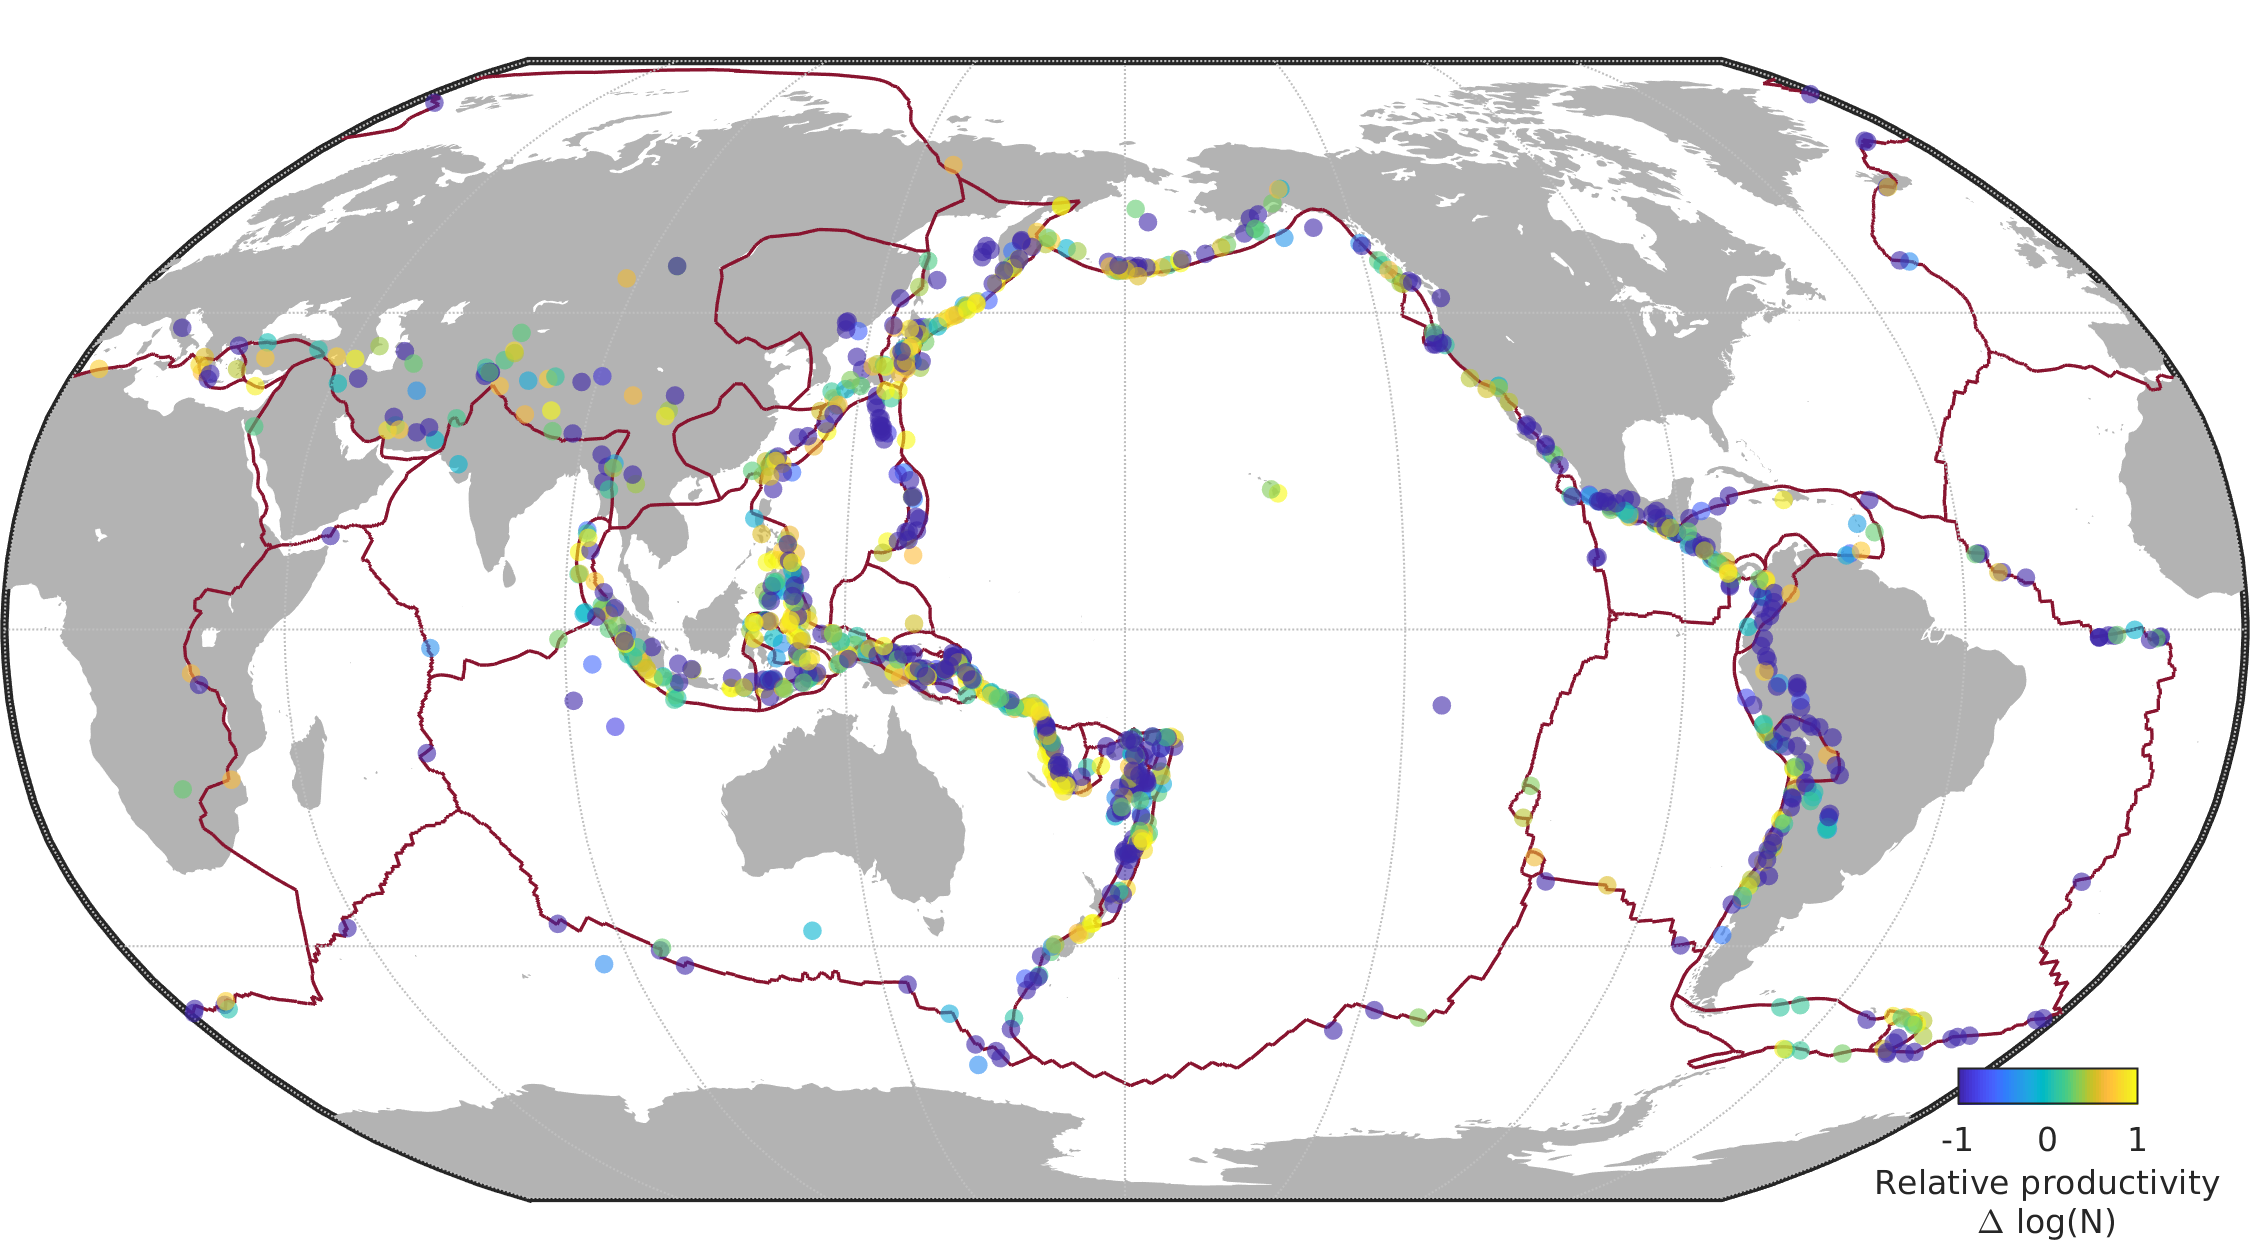
\includegraphics[width=\linewidth]{figures/worldmap_res_mw5.png}
\caption{Global map of earthquake productivity \add{as measured with a catalog completeness threshold of $M_W5.0$}. Red lines indicate the surface trace of the tectonic boundaries. Mainshocks with $M_W\ge6.5$ color-coded according to their relative productivity.
} 
\label{fig:global_res}
\end{figure}

\begin{figure}[H]
\centering
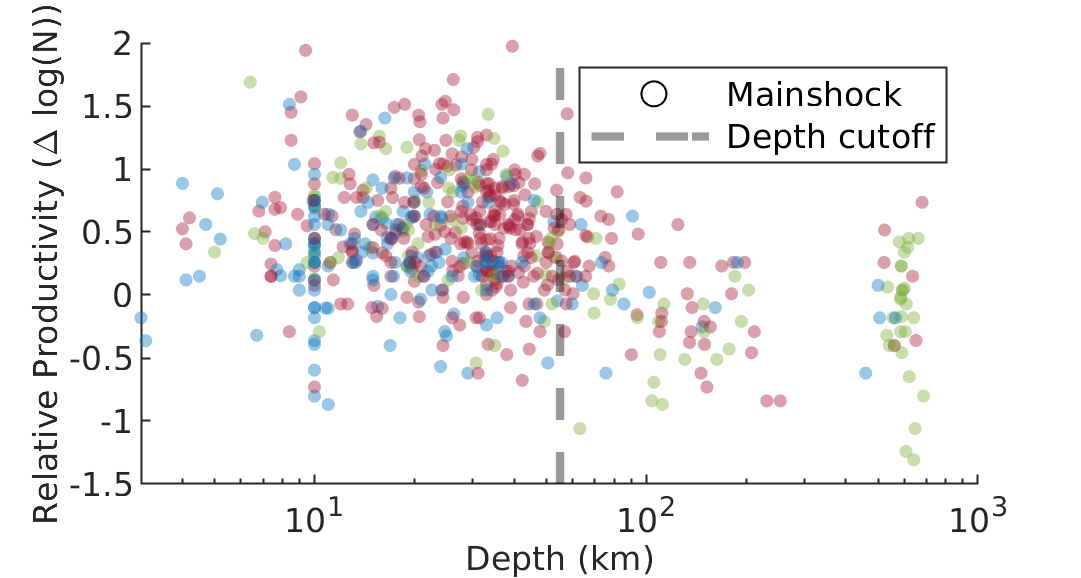
\includegraphics{figures/prod_vs_depth_mw5.png}
\caption{Relative aftershock productivity \add{measured with a catalog completeness threshold of $M_W5.0$} as a function of depth. Subsequent analysis will only consider earthquakes shallower than the 55 km cutoff (dashed line). Sequences are color-coded according to faulting style of the mainshock (blue: strike-slip, green: normal and red: reverse).}
\label{fig:prod_vs_depth}
\end{figure}


\begin{figure}[H]
\centering
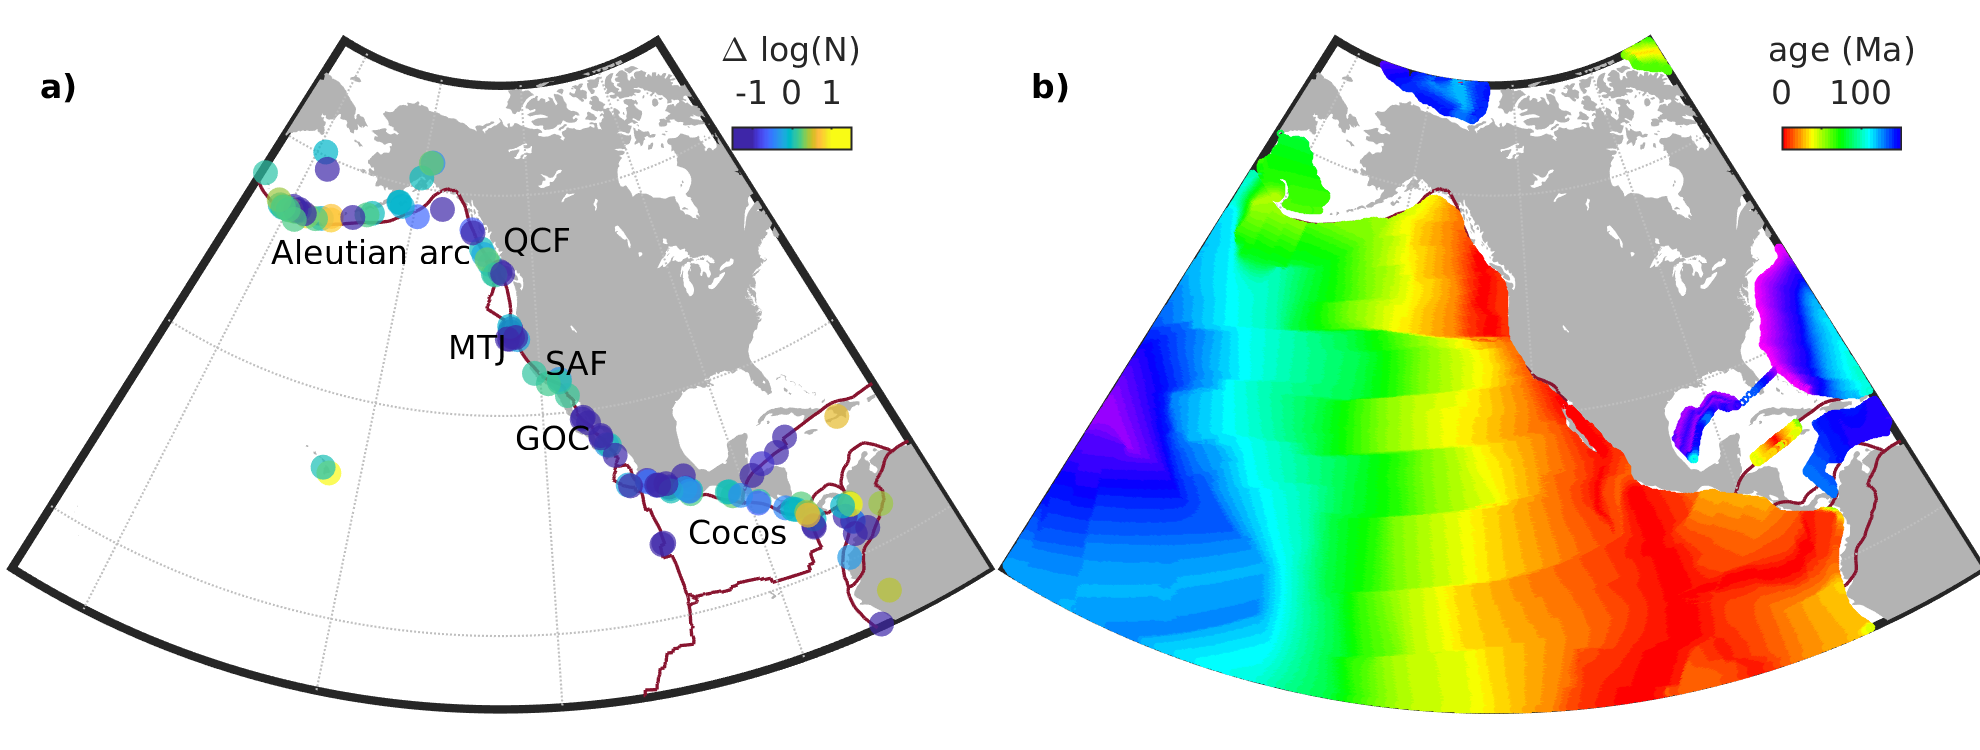
\includegraphics[width=\linewidth]{figures/regions_mw5.png}
\caption{a) Aftershock productivity \add{measured with a catalog completeness threshold of $M_W5.0$} along the North American coastline.  Individual mainshocks (points) are color-coded according to their relative aftershock productivity ($\Delta \log(N)$). The Aleutian arc, the Queen Charlotte Fault (QCF), the Mendocino Triple Junction (MTJ), San Andreas Fault (SAF), the Gulf of California (GOC) and the Cocos plate subduction include areas with coherent productivity. Red line indicates major plate boundaries \citep{Bird2003AnBoundaries}. b) Seafloor crustal age estimates from \citet{Muller2008}.}
\label{fig:region}
\end{figure}  

\begin{figure}[H]
\centering
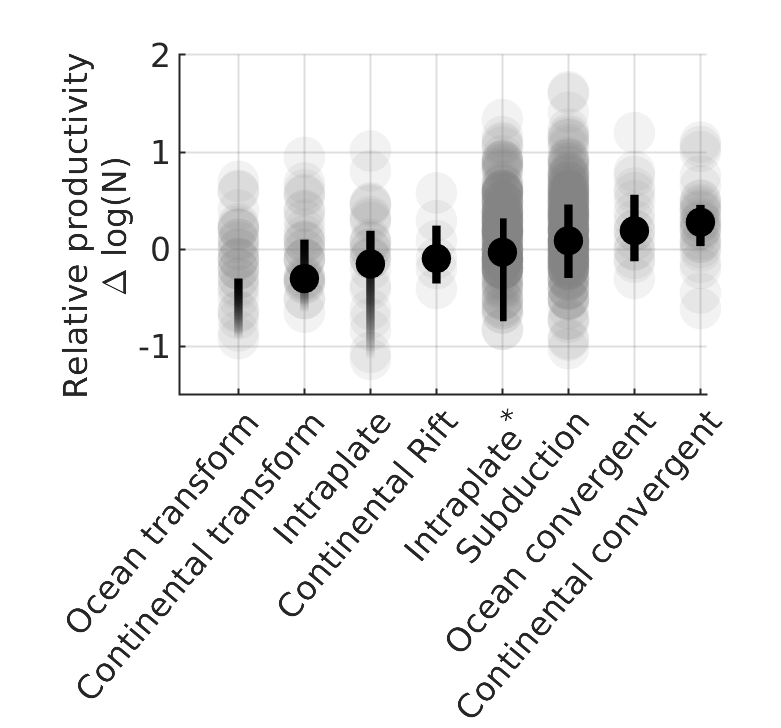
\includegraphics{figures/prod_by_pb_mw5.png}
\caption{Earthquake productivity \add{measured with a catalog completeness threshold of $M_W5.0$} by tectonic boundary. Points indicate the relative productivity of individual sequences. Solid markers and error bars indicate the median and the interquartile range. A faded lower error bar implies that mainshocks with no aftershocks are within the interquartile range. Intaplate$^*$ indicates earthquakes within 400km from a plate boundary but with a faulting mechanism discordant with the plate boundary (e.g., outer rise events).}
\label{fig:plate_boundary}
\end{figure}    


\begin{figure}[H]
\centering
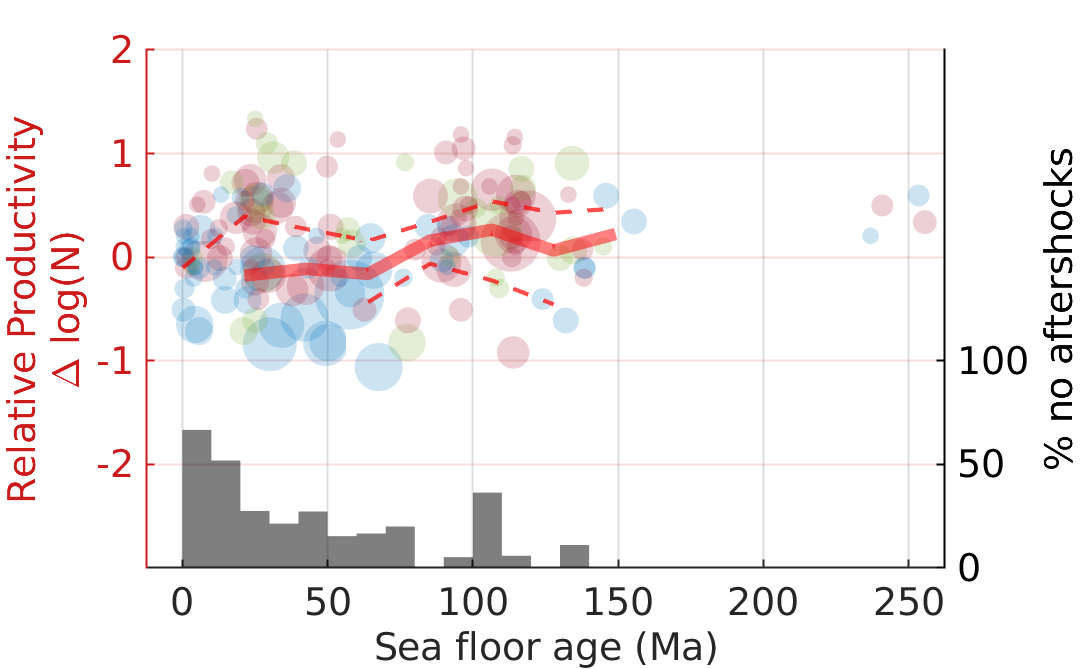
\includegraphics{figures/prod_vs_age_mw5.png}
\caption{Relative productivity \add{measured with a catalog completeness threshold of $M_W5.0$} increases as a function of the age of the oceanic lithosphere. Each point indicates an individual earthquake sequence. Sequences are color-coded by faulting style of the mainshock (blue: strike-slip, green: normal and red: reverse). The red line indicates the median average for 20Ma crustal age bins. Dashed lines indicate the corresponding interquartile ranges. Bars indicate the fraction of earthquakes with no aftershocks within each 10~Ma crustal age bin.}
\label{fig:prod_vs_age}
\end{figure}   

\begin{figure}[H]
\centering
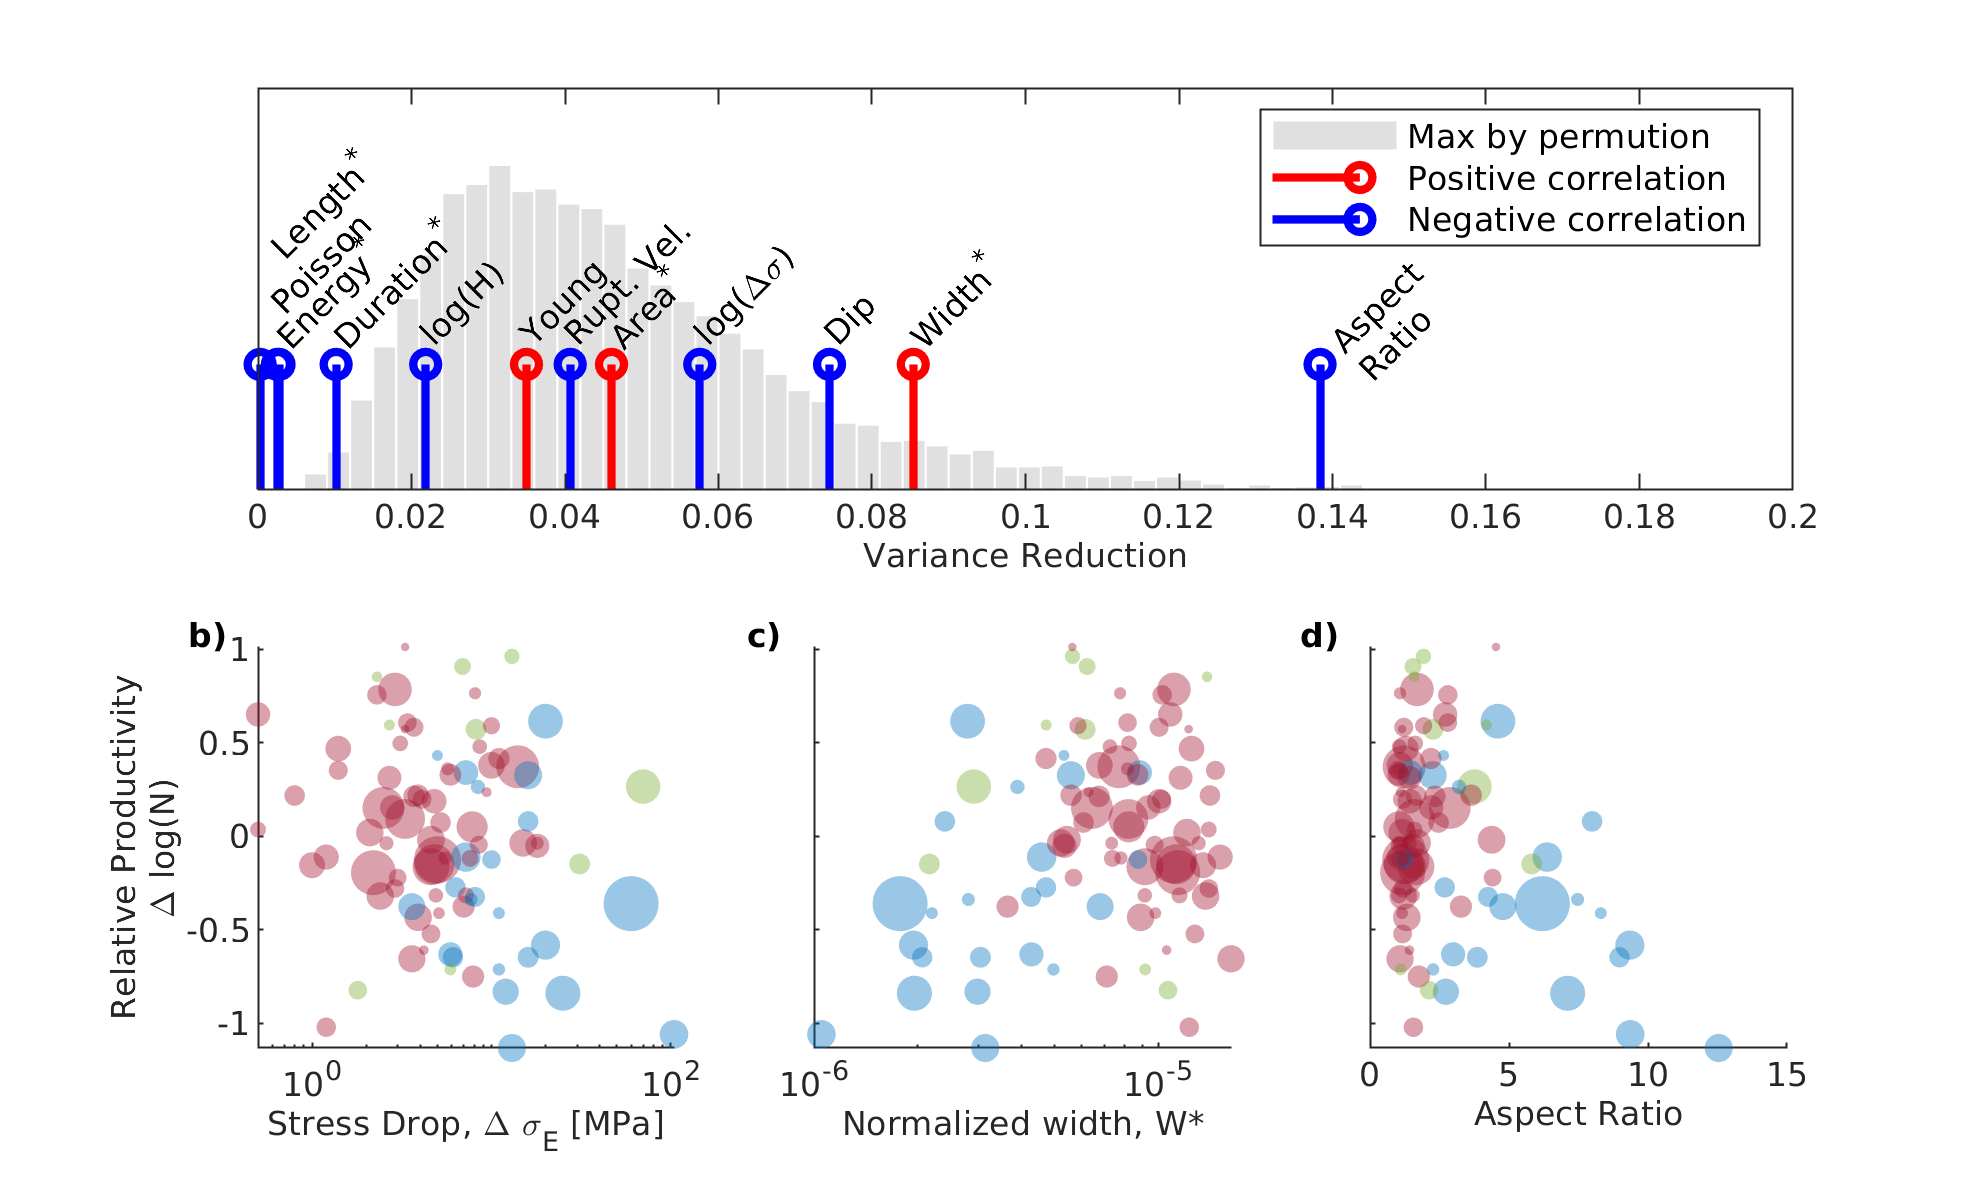
\includegraphics{figures/stem_plot_mw5.png}
\caption{\add{Inspection of the relationship between source attributes and relative productivity measure with a catalog  completeness of $M_W5$}. a) Goodness of fit of linear regressions for each source attribute in our combined catalog. Top and bottom axes respectively represent the p-value and goodness of fit of each attribute (stems). The probability distribution function in the backdrop indicates the maximal variance reduction outcome of 10000 permutation test of the entire data set. The probability of obtaining a spurious correlation by chance over the whole family of attributes we tested for is derived from the number of random shuffles exceeding the measured variance reduction and normalized to the overall sample (10000). Asterisks indicate scaled and log-transformed variables. The scaled energy, length, duration and area, material properties, velocity, dip, and stress drop ($\Delta\sigma$) of the mainshock rupture all do not yield a statistically significant ($p=0.05$) linear fit to the relative productivity; the normalized rupture width and aspect ratio of the rupture yield the best fitting linear regressions. Stems are color-coded to indicate whether the source attribute is positively (red) or negatively (blue) correlated with relative productivity. b-d): Relative earthquake productivity as a function of mainshock stress drop, normalized rupture width, and aspect ratio. Individual mainshocks are color-coded according to faulting style as in Figure \ref{fig:fms_prod}.}
\label{fig:r2_finite_fault}
\end{figure}

\begin{figure}[H]
\centering
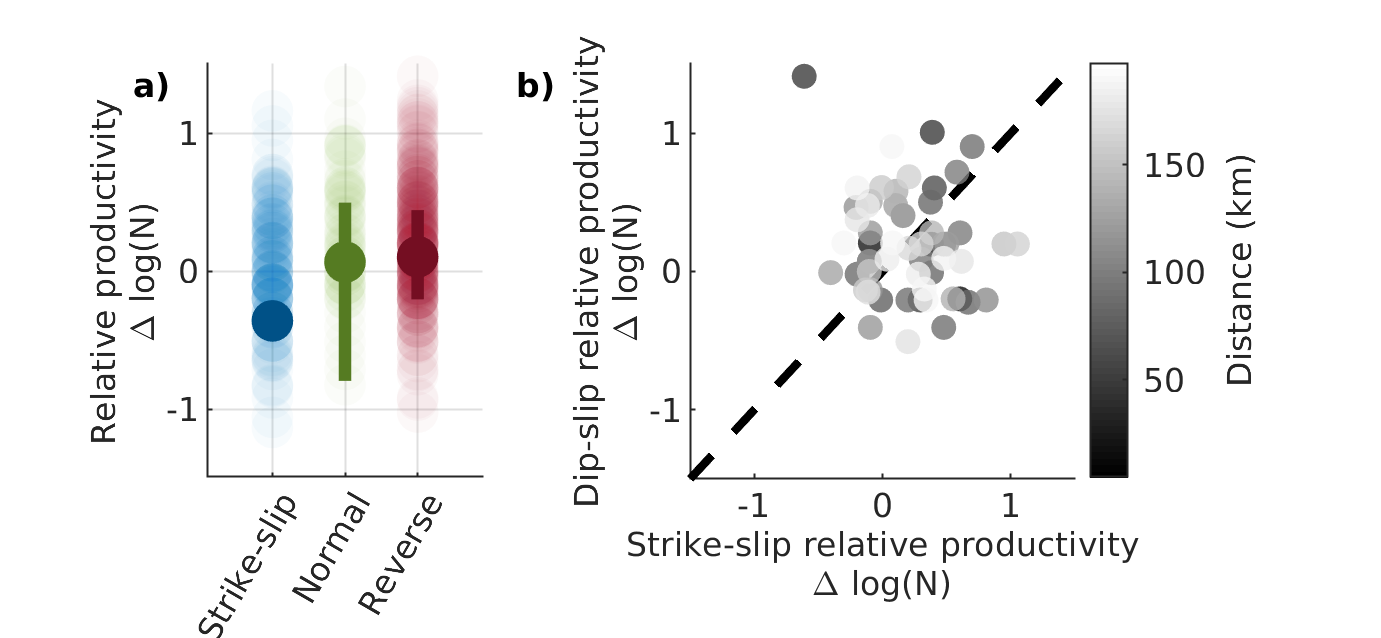
\includegraphics{figures/fmspairs_mw5.png}
\caption{\add{Inspection of the relationship between focal mechanism and relative productivity as measured with a catalog completeness threshold of $M_W5$}. a) Relative aftershock productivity ($\Delta \log(N)$) by focal mechanism. b) Relative aftershock productivity for pairs of earthquake sequences with strike-slip and dip-slip mainshocks within 200 km from each other. Each pair is shaded according to its relative distance. Dashed line indicates a 1:1 relationship, the expectation for a purely site dominated control on relative productivity. Co-located mainshocks pairs generally follow this 1:1 trend, but exhibit considerable scatter.}
\end{figure}

\begin{figure}[H]
\centering
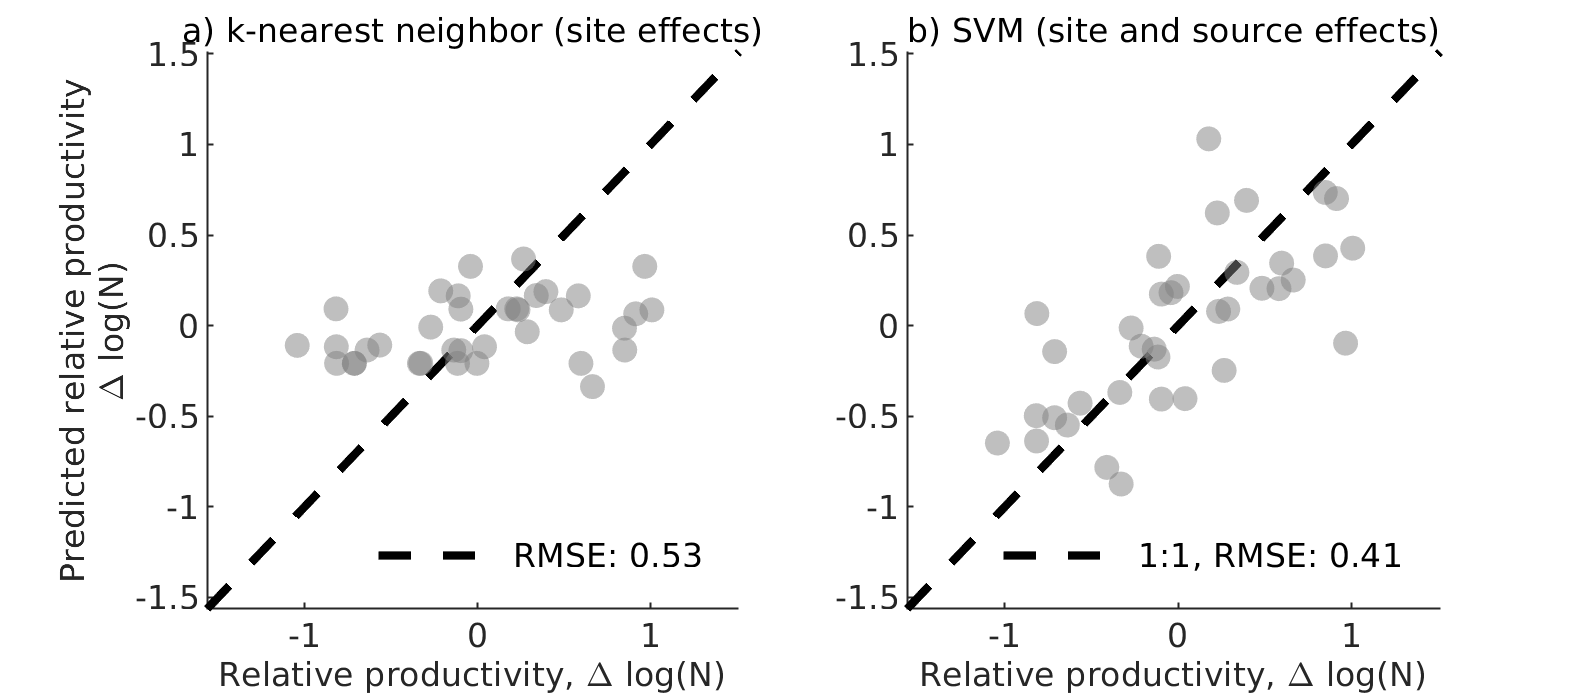
\includegraphics{figures/response_mw5.png}
\caption{\add{Sensitivity of two forecasting approaches to catalog completeness. Measurements here of relative productivity are computed using a catalog completeness of $M_W5.0$}. Response plots (prediction versus observation) for the k-nearest neighbor algorithm and SVM models. Each point is an individual earthquake sequence. A perfect prediction would place all values on the 1:1 line. The SVM model outperforms the k-nearest neighbor model. Hold-one-out cross-validation ensures that the data for model calibration is separate from the prediction data. Combining both contextual information about the setting (crustal age) and the source (dip and normalized area) yields a root mean square value of 0.39. In particularly, the SVM model better predicts extreme cases (highly productive or unproductive).}
\label{fig:response}
\end{figure}

\begin{figure}[H]
\centering

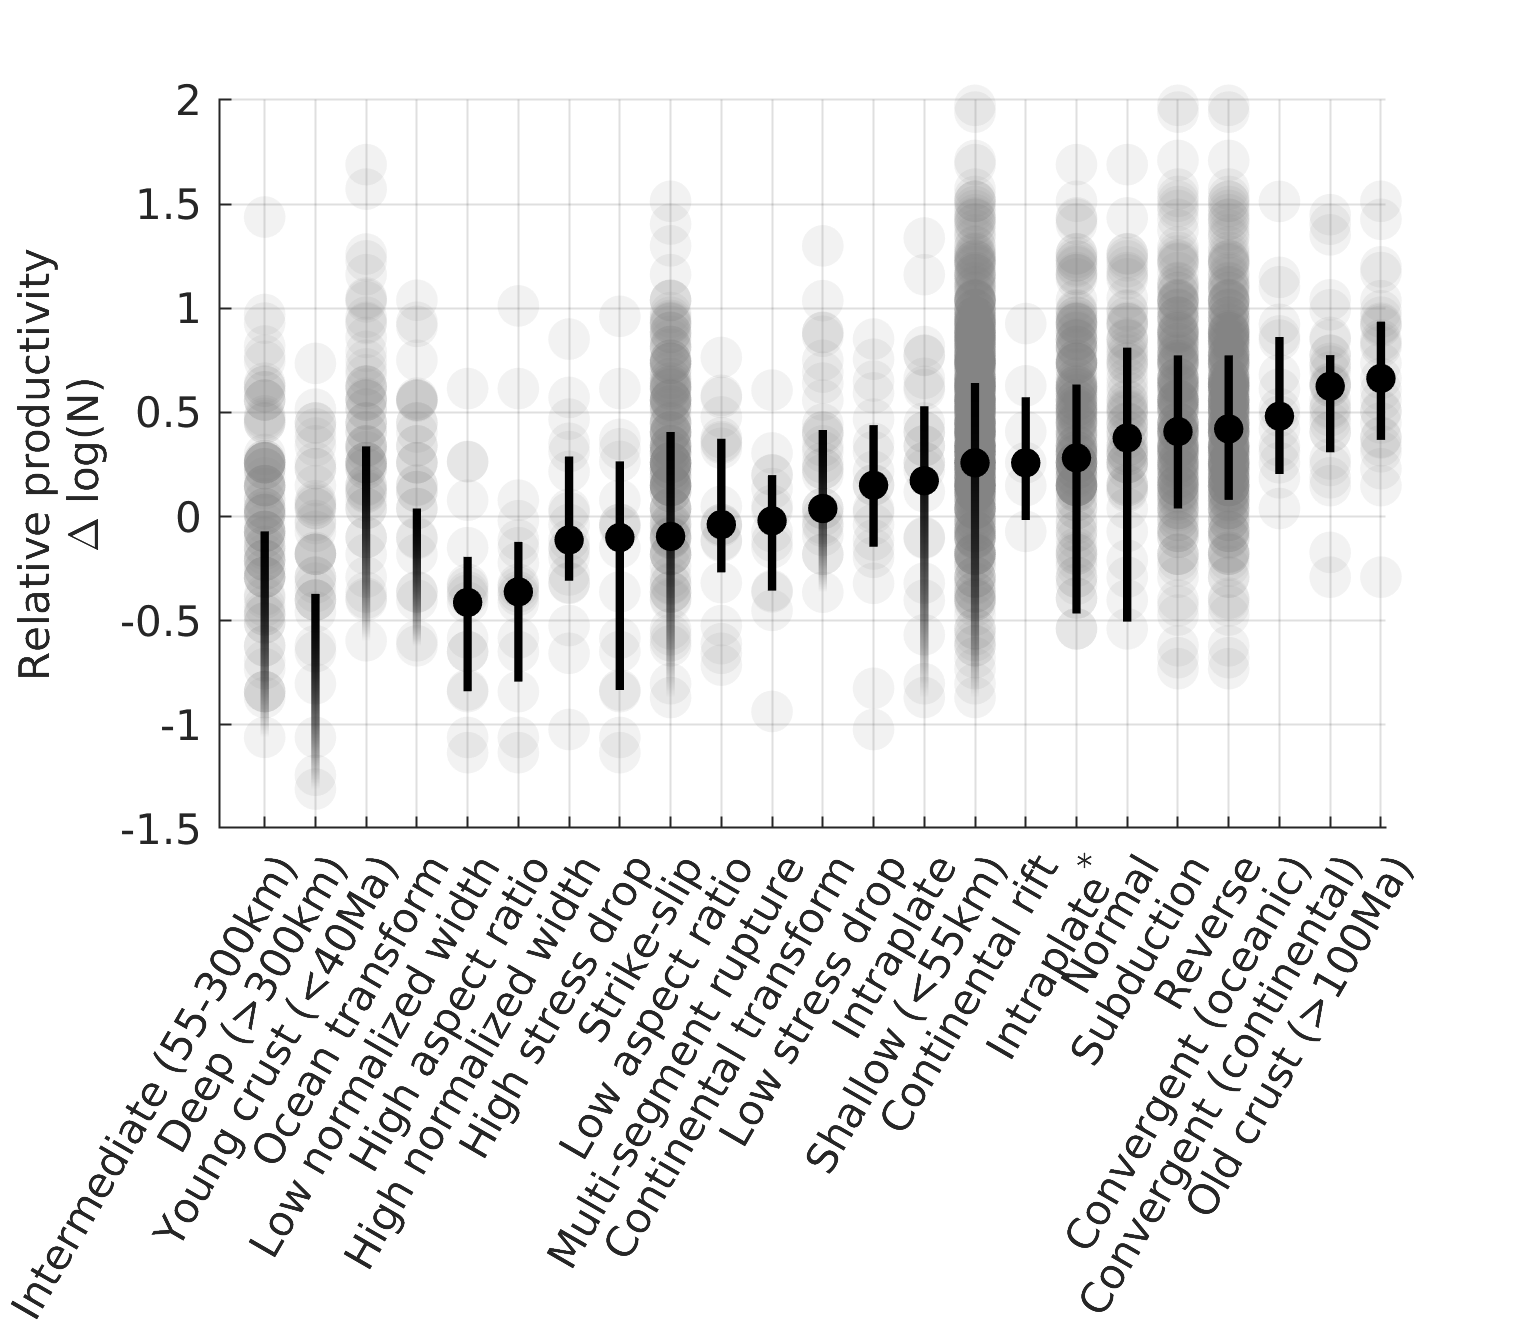
\includegraphics{figures/cal_tech_mw5.png}
\caption{Synthesis of relative productivity \add{measured with a catalog completeness threshold of $M_W5.0$} according to catalog subsets. The group considered here are the short list which best distinguished relative productivity based on our different lines of investigation. `High' and `low' subsets respectively refer to $>\!\!80$th and $<\!\!20$th percentile ranges of the data. Grey circles are individual mainshocks. Black points and error bars respectively indicate the median and interaquartile range of the subset. Fading error bars imply that mainshock sequences with no aftershocks are within the interquartile range of the data.}
\label{fig:caltech}
\end{figure}   

\newpage
\subsection{Alternative clustering method}\label{sec:alt}

%(Figures \ref{fig:method_val}-\ref{fig:caltech}) 
In this section we present the salient results of our study using an alternate clustering approach. The main manuscript presents results obtained using a hierarchical space-time windowing scheme. We preferred this method because it is more readily reproducible on an event by event basis and therefore provides  transparency.  A reader is readily capable of inspecting individual past or future earthquakes to see where they fall with respect to the global average, and whether they corroborate or challenge our conclusions without having to perform extensive additional calculations. However, it is important to also check the result robustness with more mathematically rigorous aftershock detection methods.   

Here we present our major results using aftershock counts obtained following \citet{Zaliapin2008}. This approach seeks to build earthquake families by linking earthquakes to parent events. Separation of clusters is achieved by finding a decision boundary between background events and clustered events. See \citet{Zaliapin2008} for a detailed overview of the method, distance metrics, and theoretical connections to other schemes (ETAS). Though there are discrepancies, aftershock counts obtained using this method correspond well to counts obtained using space-time windowing (see Figure \ref{fig:method_val}). Additionally, we find few differences to the major results of the study (see Figure \ref{fig:fms_prod2_z2008}--\ref{fig:caltechzaliapin}).
The workflow and detailed explanations of the clustering routine are available here: https://github.com/tgoebel/clustering-analysis.

%%%%%%%%%%%%%%%%%%%%%%%%%%%%%%%%%%%%%%%%%%%%%%%%%%%%%%%%%%%%%%%%%%%%%%%%%%%%%%%%%%%%%%%%%%%%%%%%%%%%%%%%%%%%%%%%%%%%%%%%%%%%%%%%%%%%%%%%%%%%%%%%%%%%%%%%%%%%%%%%%%%%%%%%%%%%%%%%%%%%%%%%%%%%%%%%%%%%%%%%%%%%%%%%%%%%%%%%

\begin{figure}[H]
\centering
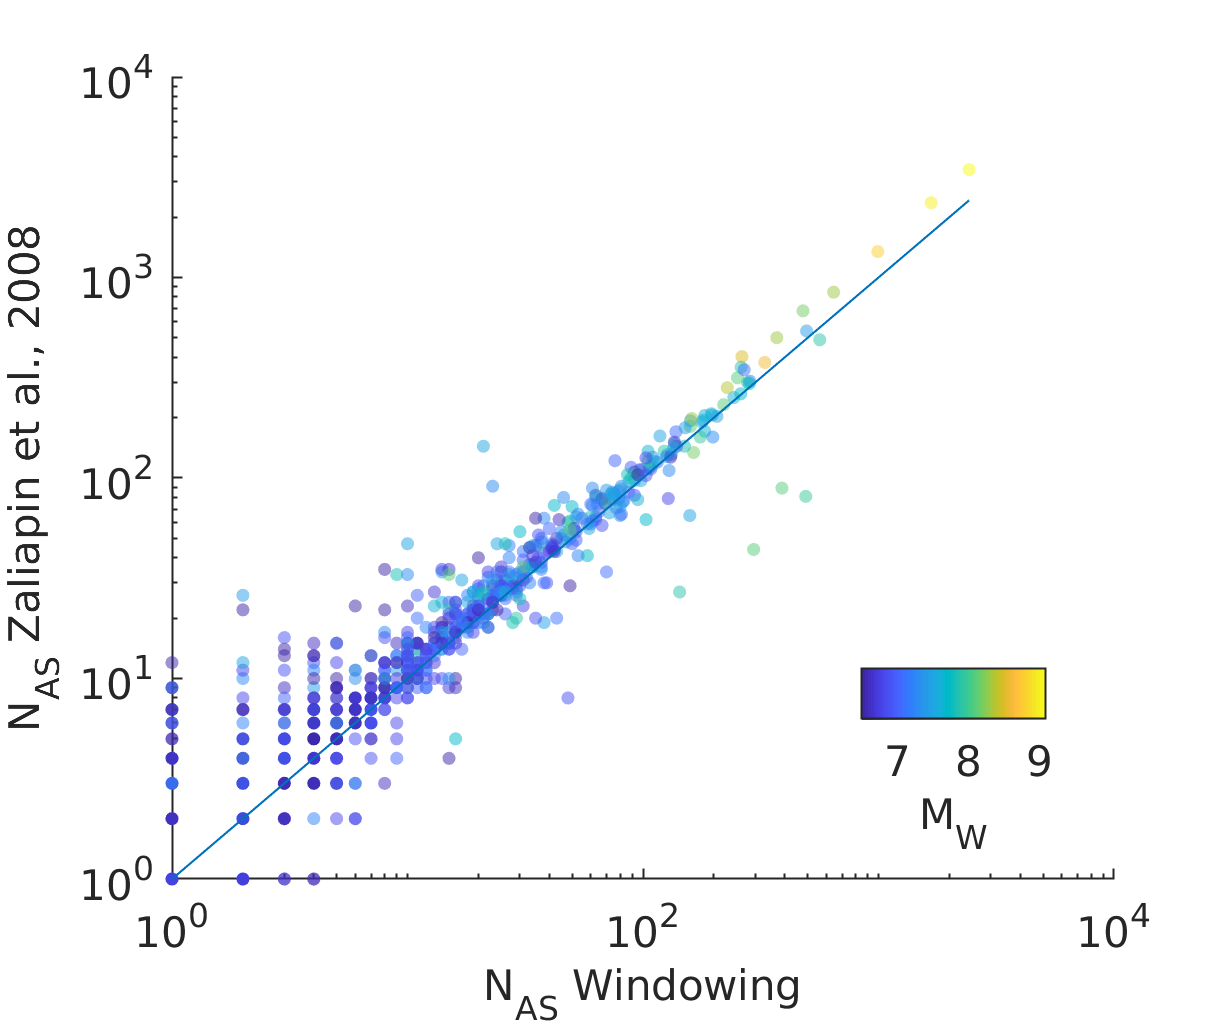
\includegraphics{figures/method_validation.png} 
\caption{Comparison of aftershock counts obtained using space time windowing and those obtained using nearest neighbor clustering \citep[following][]{Zaliapin2008}. Each point represents an individual mainshock. Mainshocks are colored according to moment magnitude. Blue line indicates a 1 to 1 correspondence.}
\label{fig:method_val}
\end{figure}

%%%%%%%%%%%%%
\begin{figure}[H]
    \centering
        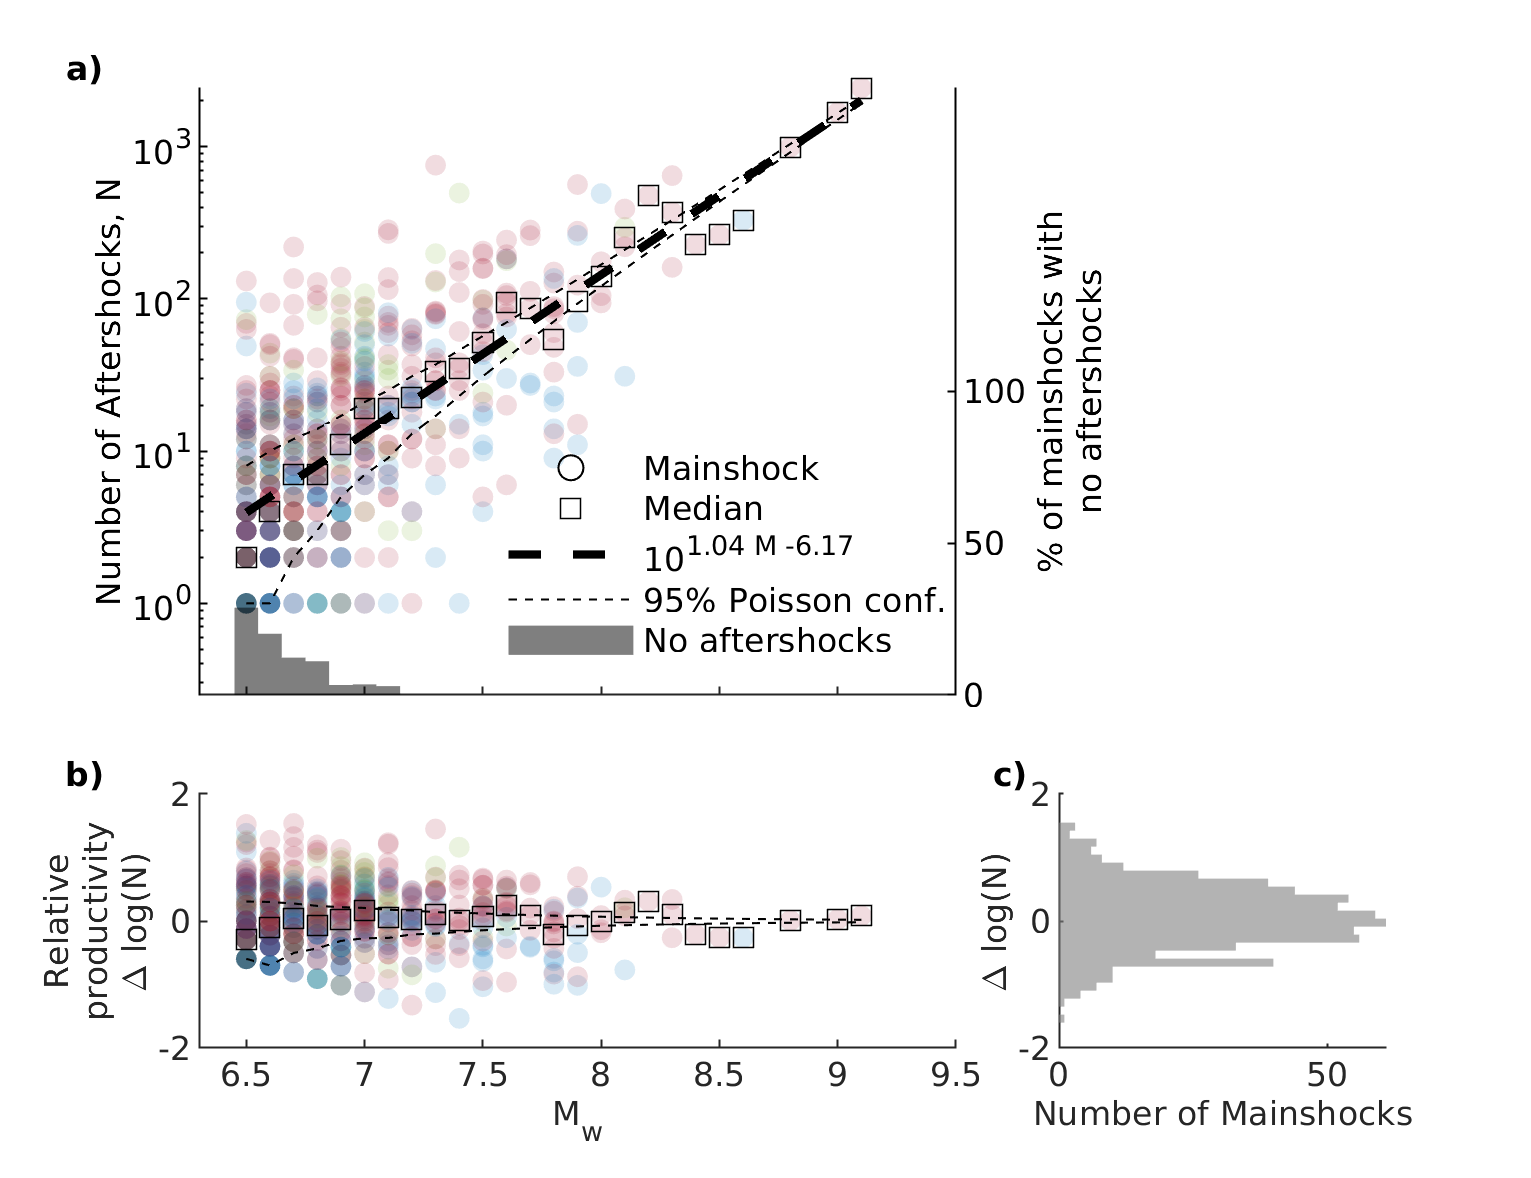
\includegraphics{figures/prod_law_z2008.png}
    
    \caption{Results using \citet{Zaliapin2008} clustering. a) The number of aftershocks of $M_W\ge4.5$ within three source dimensions and 60 days as a function of mainshock magnitude identified in the global ISC and NEIC catalogs from 1990 to 2019. Colors indicate faulting style of the mainshock; blue, green and red points correspond to earthquake sequences for which the mainshock was respectively strike-slip, normal or reverse. The global productivity law (dashed line) is fit using a least squares regression through the median log-number of aftershocks for each 0.1 magnitude bin (black squares). The median number includes mainshocks with no aftershocks which are not shown on the plot. Individual earthquake sequences (circles) scatter significantly above and below the productivity law. b) Relative productivity (Eq.~5) as a function of mainshock magnitude. The relative productivity distribution does not show events with no aftershocks and thus the lower left corner of the plot is underpopulated. c) Histogram of the relative productivity of mainshocks considered in this study.
    }
    \label{fig:fms_prod2_z2008}
\end{figure}

%%%%%%%%%%%%%%%%%%%%%%%%%%%%%%%%%%%%%%%%%%%%%%%%%%%%%

\begin{figure}[H]
    \centering

        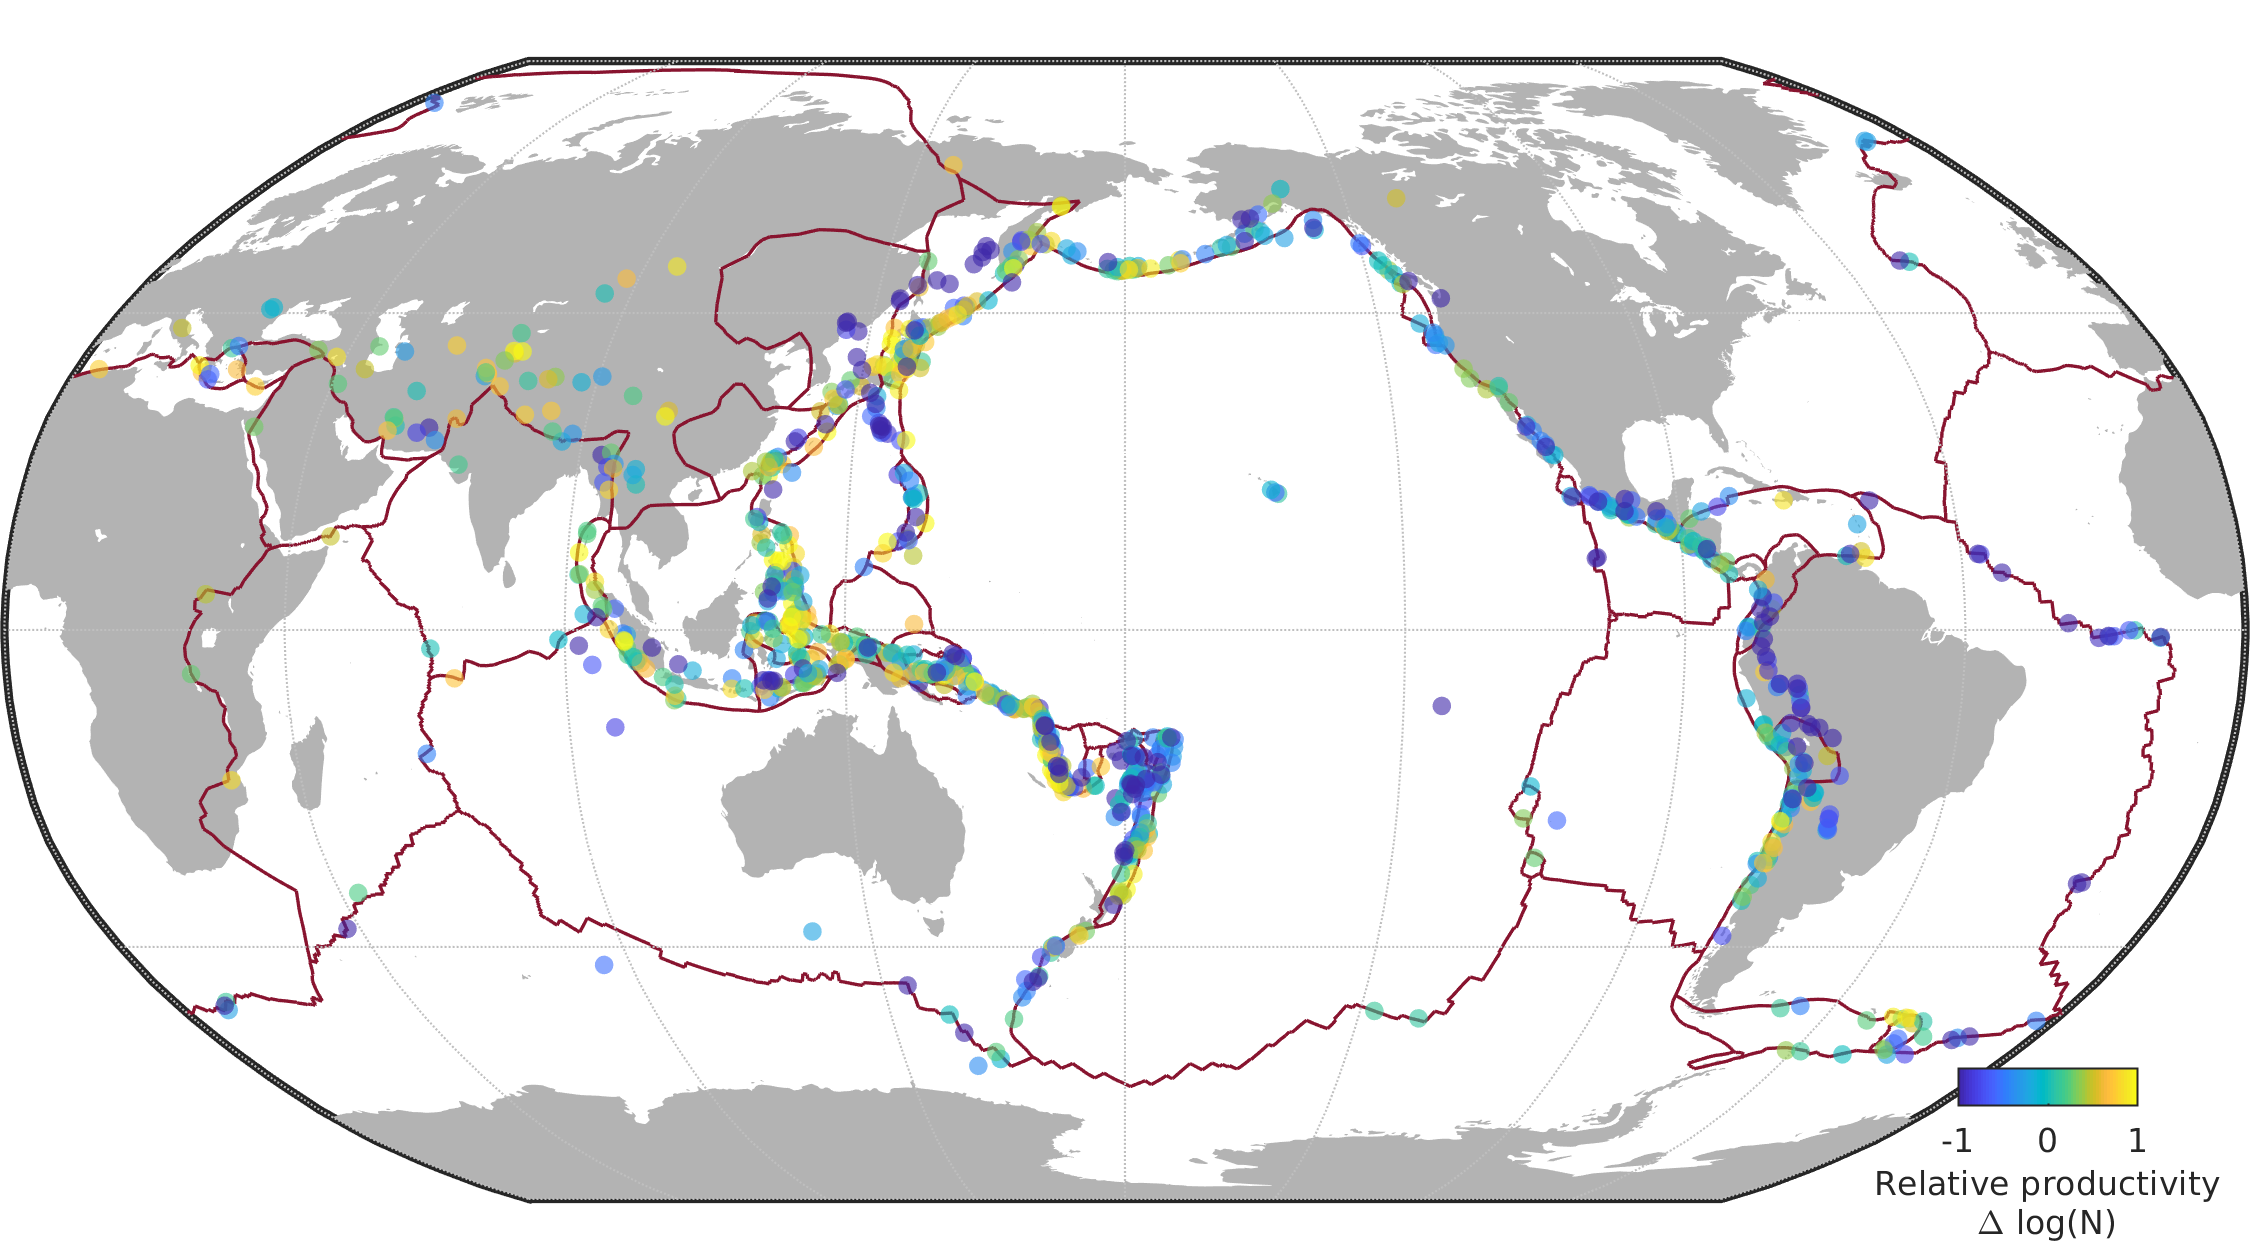
\includegraphics[width = \linewidth]{figures/worldmap_res_z2008.png}
    
    \caption{Results using \citet{Zaliapin2008} clustering. Global map of earthquake productivity. Red lines indicate the surface trace of the tectonic boundaries. Mainshocks with $M_W\ge6.5$ color-coded according to their relative productivity (Equation 5)}
\end{figure}

%%%%%%%%%%%%%%%%%%%%%%%%%%%%%%%%%%%%%%%%%%%%%%%%%%%%%

\begin{figure}[H]
    \centering

        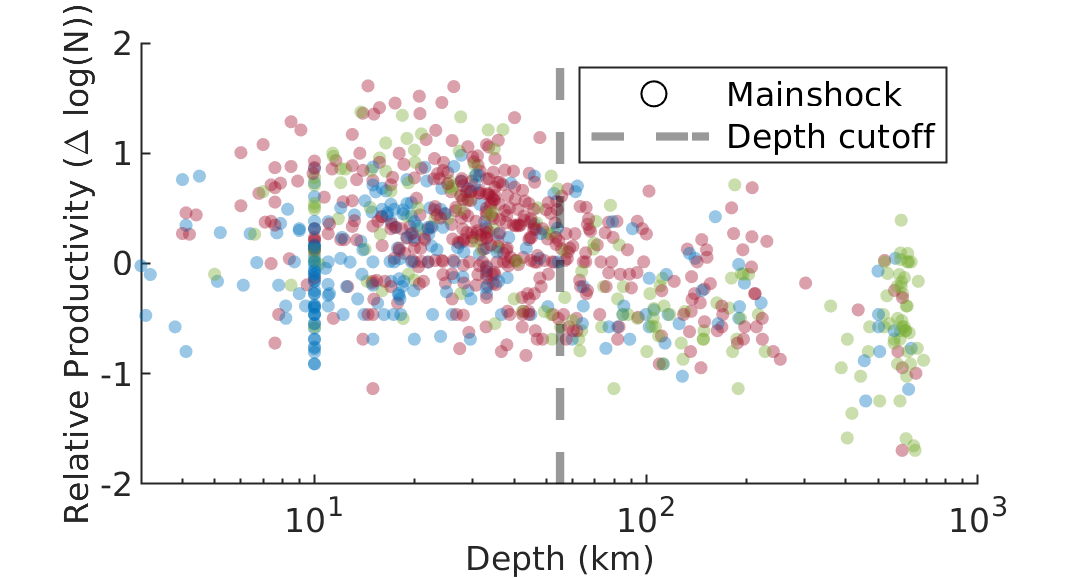
\includegraphics{figures/prod_vs_depth_z2008.png}
    
    \caption{Results using \citet{Zaliapin2008} clustering. Relative aftershock productivity as a function of depth. Subsequent analysis will only consider earthquakes shallower than the 55 km cutoff (dashed line). Sequences are color-coded according to faulting style of the mainshock (blue: strike-slip, green: normal and red: reverse). Note: Discretization of depth is apparent in this plot as some events have default values. Depths of  33~km, 5~km, 10~km and 15~km are reported for  6\%, 1\%, 10\% and 0.7\%, respectively, of the catalog.}
\end{figure}

%%%%%%%%%%%%%%%%%%%%%%%%%%%%%%%%%%%%%%%%%%%%%%%%%%%%

\begin{figure}[H]
    \centering

        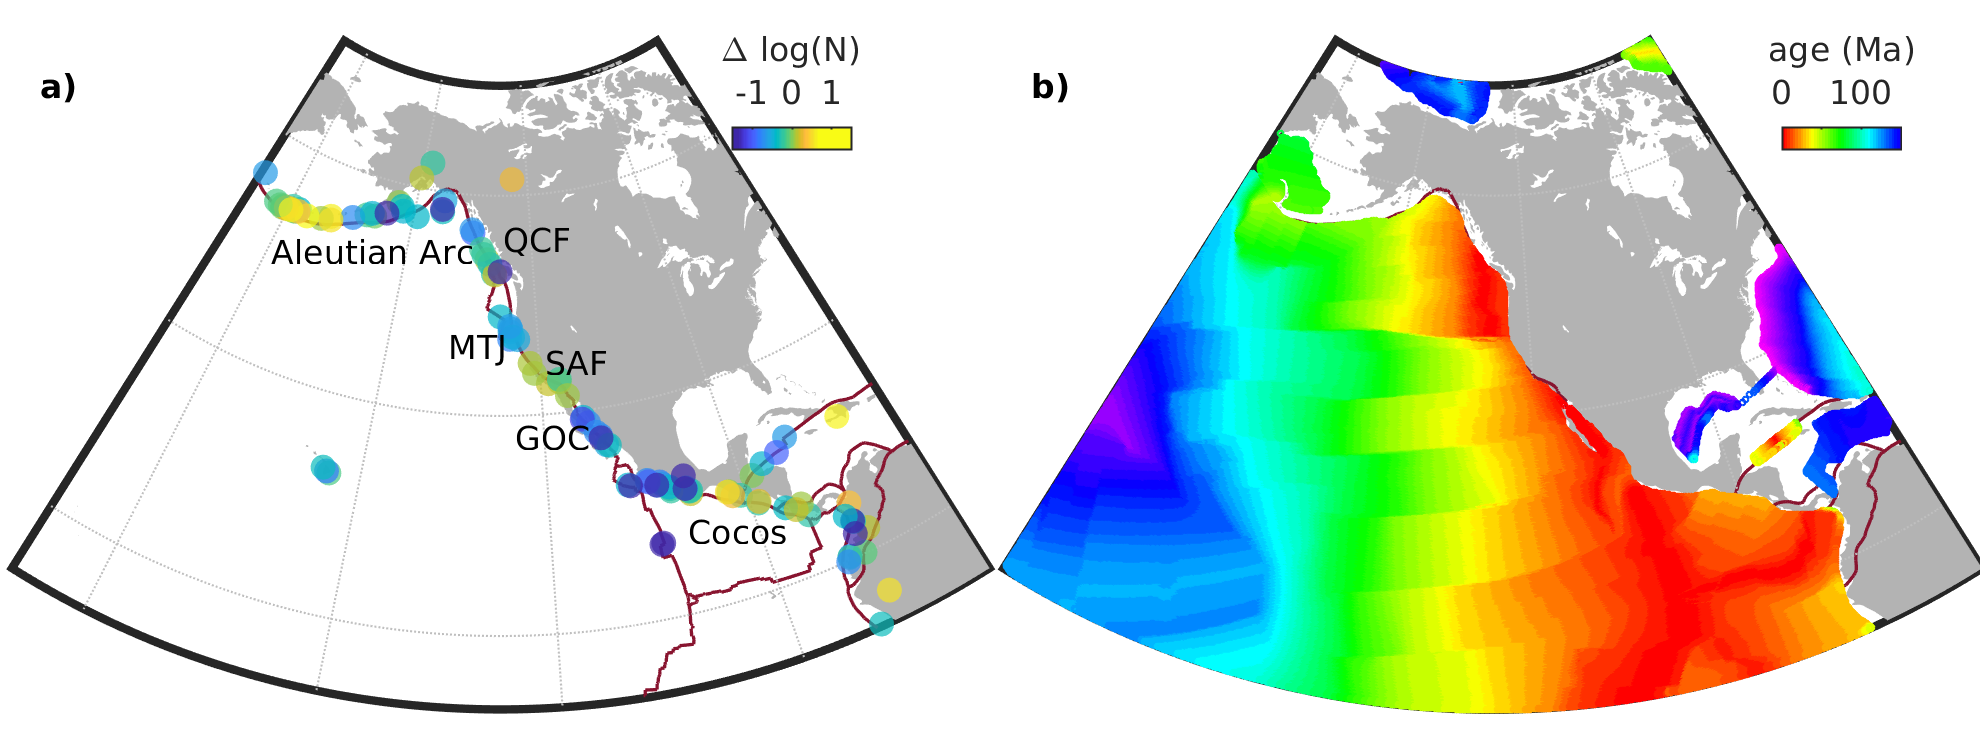
\includegraphics[width = \linewidth]{figures/regions_z2008.png}
    
    \caption{Results using \citet{Zaliapin2008} clustering. a) Aftershock productivity along the North American coastline.  Individual mainshocks (circles) are color-coded according to their relative aftershock productivity. The Aleutian Arc, Queen Charlotte Fault (QCF), Mendocino Triple Junction (MTJ), San Andreas Fault (SAF), Gulf of California (GOC) and Cocos Plate Subduction Zone include areas with coherent productivity. Red line indicates major plate boundaries \citep{Bird2003AnBoundaries}. b) Seafloor crustal age estimates from \citet{Muller2008}.}
\end{figure}

%%%%%%%%%%%%%%%%%%%%%%%%%%%%%%%%%%%%%%%%%%%%%%%%%%%%%

\begin{figure}[H]
    \centering

        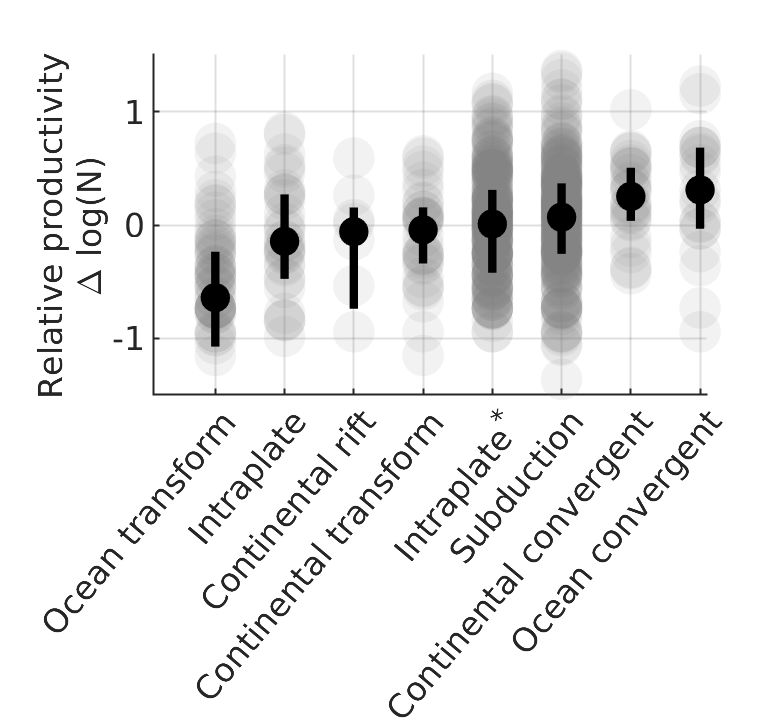
\includegraphics{figures/prod_by_pb_z2008.png}
    
    \caption{Results using \citet{Zaliapin2008} clustering. Earthquake productivity by tectonic boundary. Circles indicate the relative productivity of individual sequences. Solid markers and error bars indicate the median and the interquartile range. A faded lower error bar implies that mainshocks with no aftershocks are within the interquartile range. Intraplate$^*$ indicates earthquakes within 400 km of a plate boundary but with a faulting mechanism discordant with the plate boundary (e.g., outer rise events).}
        \label{fig:plate_boundary_z2008}
\end{figure}
%%%%%%%%%%%%%%%%%%%%%%%%%%%%%%%%%%%%%%%%%%%%%%%%%%%%%

\begin{figure}[H]
    \centering

        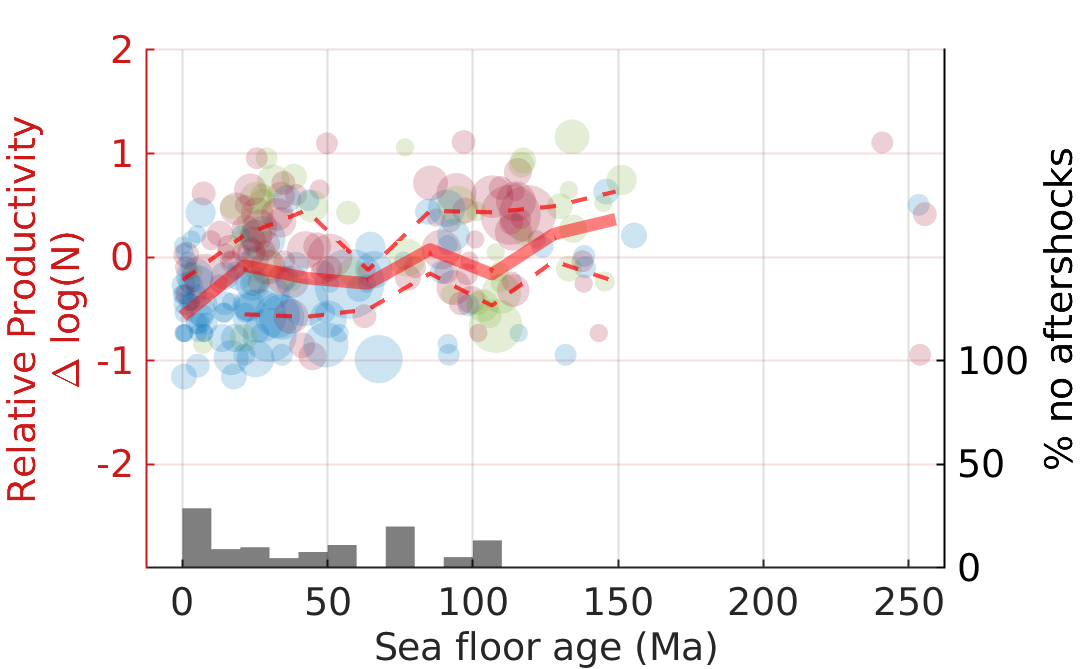
\includegraphics{figures/prod_vs_age_z2008.png}
    
    \caption{Results using \citet{Zaliapin2008} clustering. Relative productivity increases as a function of the age of the oceanic lithosphere. Each circle indicates an individual earthquake sequence. Sequences are color-coded by faulting style of the mainshock (blue: strike-slip, green: normal and red: reverse). The red line indicates the median average for 20~Ma crustal age bins. Dashed lines indicate the corresponding interquartile ranges. Bars indicate the fraction of earthquakes with no aftershocks within each 10Ma crustal age bin and correspond to the right-hand axis.}
        \label{fig:prod_vs_age_z2008}
\end{figure}

%%%%%%%%%%%%%%%%%%%%%%%%%%%%%%%%%%%%%%%%%%%%%%%%%%%%%

\begin{figure}[H]
    \centering
        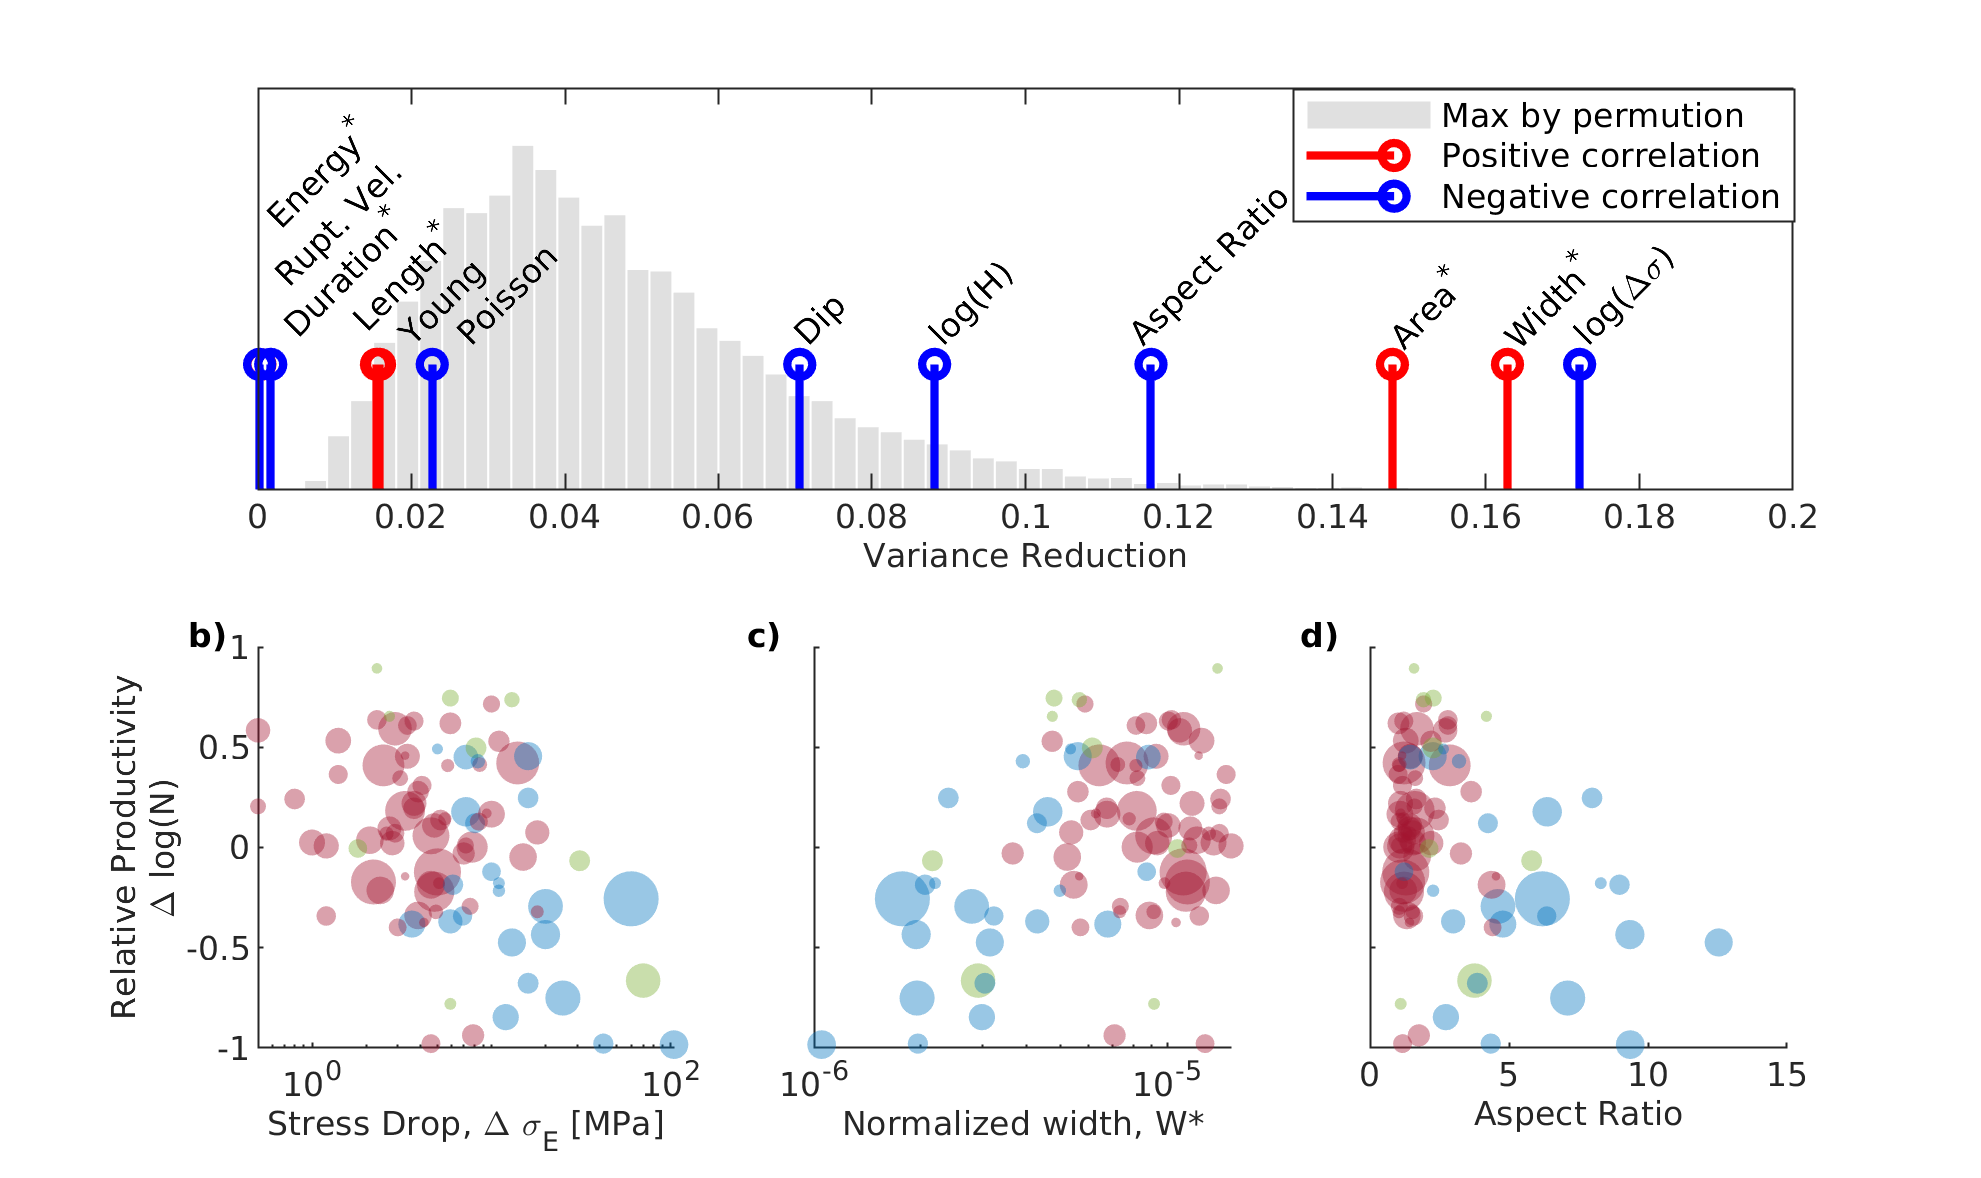
\includegraphics[width = 0.8\linewidth]{figures/stem_plot_z2008.png}
    
    \caption{Results using \citet{Zaliapin2008} clustering. a) Goodness of fit of linear regressions for each source attribute in our combined catalog. Top and bottom axes respectively represent the p-value and goodness of fit of each attribute (stems). The probability distribution function in the backdrop indicates the maximal variance reduction outcome of 10000 permutation test of the entire data set we tested. Asterisks indicate scaled and log-transformed variables. The scaled energy, length, duration and area, material properties, velocity, dip, and log-stress drop ($\Delta\sigma$) of the mainshock rupture all do not yield a statistically significant ($p=0.05$) linear fit to the relative productivity — the normalized rupture width and aspect ratio of the rupture yield the best fitting linear regressions. Stems are color-coded to indicate whether the source attribute is positively (red) or negatively (blue) correlated with relative productivity. b-d): Relative earthquake productivity as a function of mainshock stress drop, normalized rupture width, and aspect ratio.}
        \label{fig:r2_finite_fault_z2008}
\end{figure}

%%%%%%%%%%%%%%%%%%%%%%%%%%%%%%%%%%%%%%%%%%%%%%%%%%%%%

\begin{figure}[H]
    \centering

        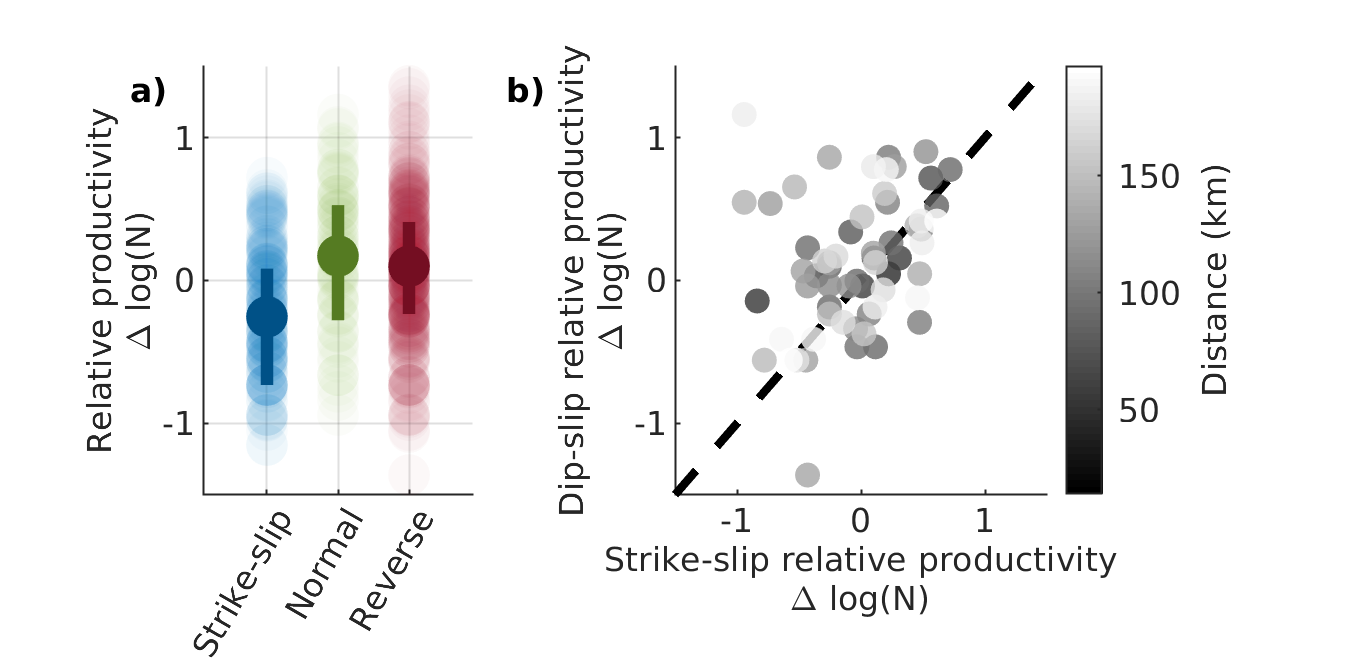
\includegraphics{figures/fmspairs_z2008.png}
    
    \caption{Results using \citet{Zaliapin2008} clustering. a) Relative aftershock productivity ($\Delta \log(N)$ by focal mechanism (Equation 5). b) Relative aftershock productivity for pairs of earthquake sequences with strike-slip and dip-slip mainshocks within 200 km from each other. Each pair is shaded according to its relative distance. Dashed line indicates a 1:1 relationship, the expectation for a purely site dominated control on relative productivity. Co-located mainshocks pairs generally follow this 1:1 trend, but exhibit considerable scatter.}
        \label{fig:coloc_z2008}
\end{figure}
%%%%%%%%%%%%%%%%%%%%%%%%%%%%%%%%%%%%%%%%%%%%%%%%%%%%
\begin{figure}[H]
    \centering

        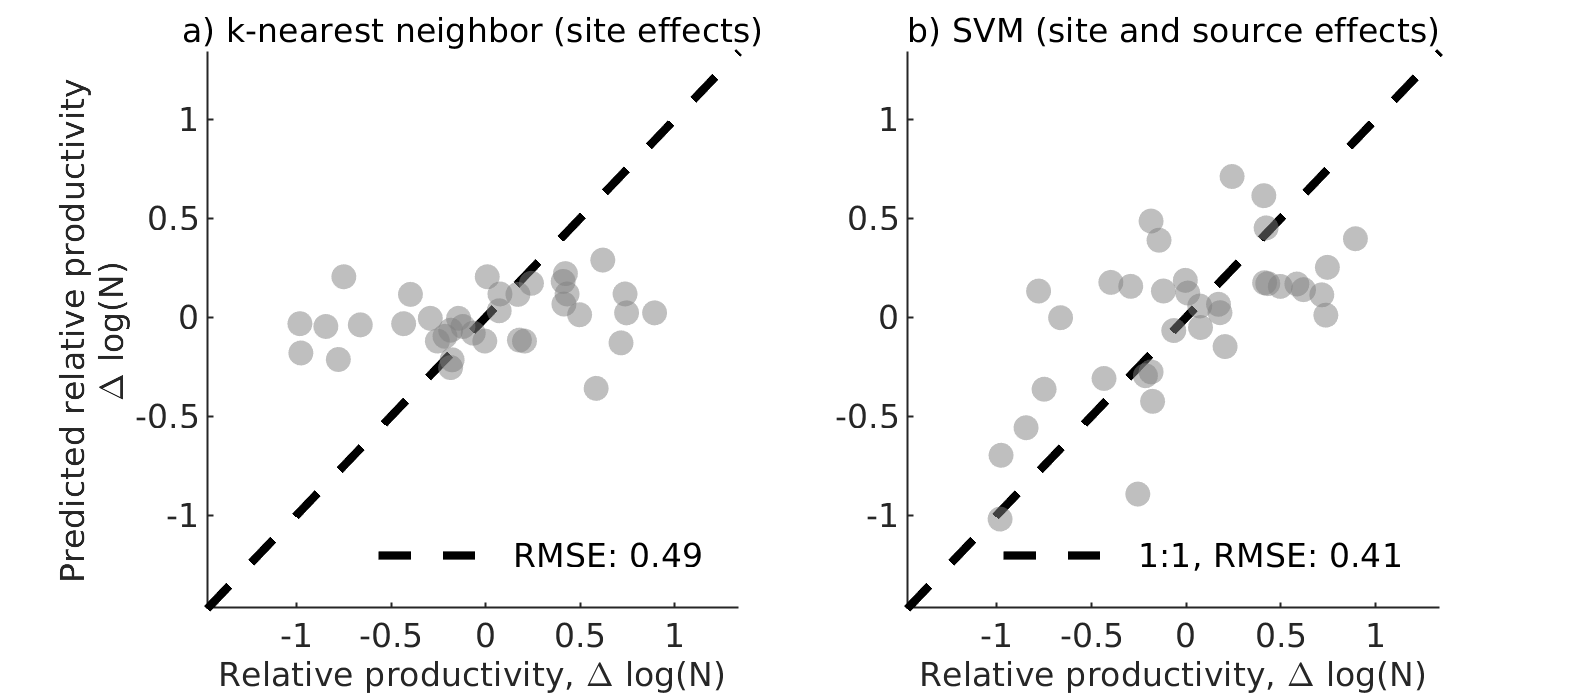
\includegraphics{figures/response_z2008.png}
    
    \caption{Results using \citet{Zaliapin2008} clustering. Response plots (prediction versus observation) for the k-nearest neighbor algorithm (a) and SVM models (b). Each point indicates prediction of relative productivity relative to that which was observed for individual earthquake sequences. A perfect prediction would place all values on the 1:1 line.}
        \label{fig:response_z2008}
\end{figure}

%%%%%%%%%%%%%%%%%%%%%%%%%%%%%%%%%%%%%%%%%%%%%%%%%%%%
\begin{figure}[H]
    \centering

        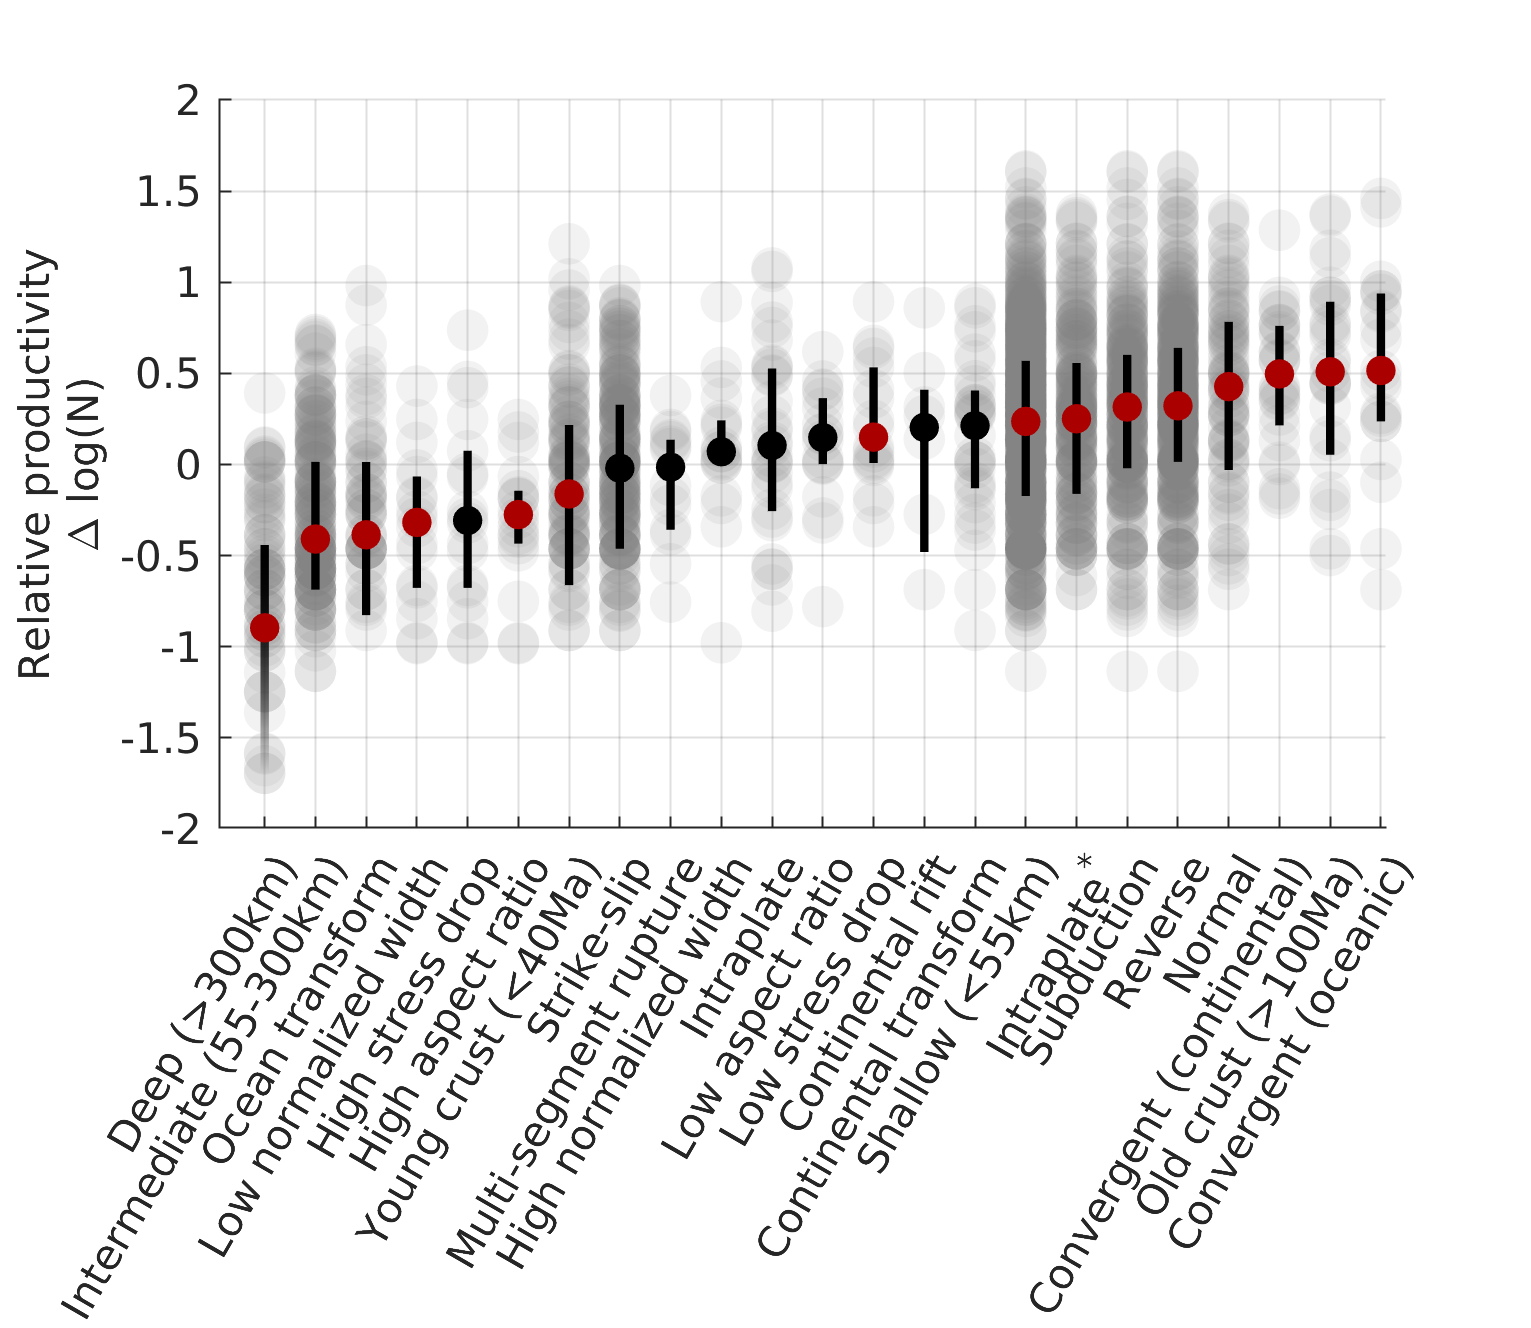
\includegraphics[width=0.6\linewidth]{figures/cal_tech_z2008.png}
    
    \caption{Results using \citet{Zaliapin2008} clustering. Synthesis of relative productivity according to catalog subsets. The group considered here are the short list which best distinguished relative productivity based on our different lines of investigation. `High' and `low' subsets respectively refer to $>\!\!80$th and $<\!\!20$th percentile ranges of the data. Grey circles are individual mainshocks. Opaque points and error bars respectively indicate the median and interaquartile range of the subset. Fading error bars imply that mainshock sequences with no aftershocks are within the interquartile range of the data. Attributes with red markers are consistent with the hypothesis that they are sample from a different continuous distribution than the overall population of earthquakes using a 2-sample Kolmogorov-Smirnov test at a 5\% significance threshold.}
        \label{fig:caltechzaliapin}
\end{figure}


%%%%%%%%%%%%%%%%%%%%%%%%%%%%%%%%%%%%%%%%%%%%%%%%%%%%%%%%%%%%%%%%%%%%%%%%%%%%%%%%%%%%%%%%%%%%%%%%%%%%%%%%%%%%%%%%%%%%%%%%%%%%%%%%%%%%%%%%%%%%%%%%%%%%%%%%%%%%%%%%%%%%%%%%%%%%%%%%%%%%%%%%%%%%%%%%%%%%%%%%%%%%%%%%%%%%%

\subsection{Background Seismicity}\label{sec:background}

Since our selection criteria for aftershocks is magnitude dependent, there is a concern that aftershock counts will be biased by background seismicity. In this section, we show that the background rate of seismicity is in fact negligible and within counting error of a Poisson process.

Measuring background seismicity is challenging and an ongoing topic of research. Approaches to measure this quantity include modelling the earthquake process as an epidemic type sequence with a stationary background rate and various declustering algorithms. However, these methods suffer from instability, subjectivity and are subject to strong trade-off between precision (granularity) and accuracy. In the extreme, event-wise calibration of background seismicity is particularly under constrained. Background seismicity is also critically dependent on the duration of an aftershock sequence (if we let aftershock sequences continue to infinity, background vanishes). Fundamentally, background estimation is sensitive to the definition of a declustering method. 

Here, we circumvent these problems by considering all events (including aftershocks) to produce an apparent background rate. We then compare this apparent background rate of events to aftershock counts. This is a conservative approach since the apparent background rate may include aftershocks that would not abide to a strict definition of background seismicity. 

Figure 2 in the manuscript shows how the aftershock-counts compare to a catalog where temporal information has been shuffled. The spatial structure, however, is conserved. This test is both a means to optimize the choice of space-time window but also an absolute upper-bound of the effect background seismicity as a function of magnitude. The effect is indeed scale dependent. However, comparing this effect to the  aftershock counts reveals that the bias is small, typically 1 to 2 orders of magnitude below the aftershock counts. Figure \ref{fig:error_comparasion} demonstrates that the bias from background seismicity lies within one standard deviation of a Poisson counting error for 97\% of mainshocks. Again, this calculated bias is an absolute upper-bound which includes aftershocks and likely a significant overestimate of background activity. The occurrence of $M_W4.5$ events in a specific small space and time window is very rare. 

\begin{figure}[H]
\centering
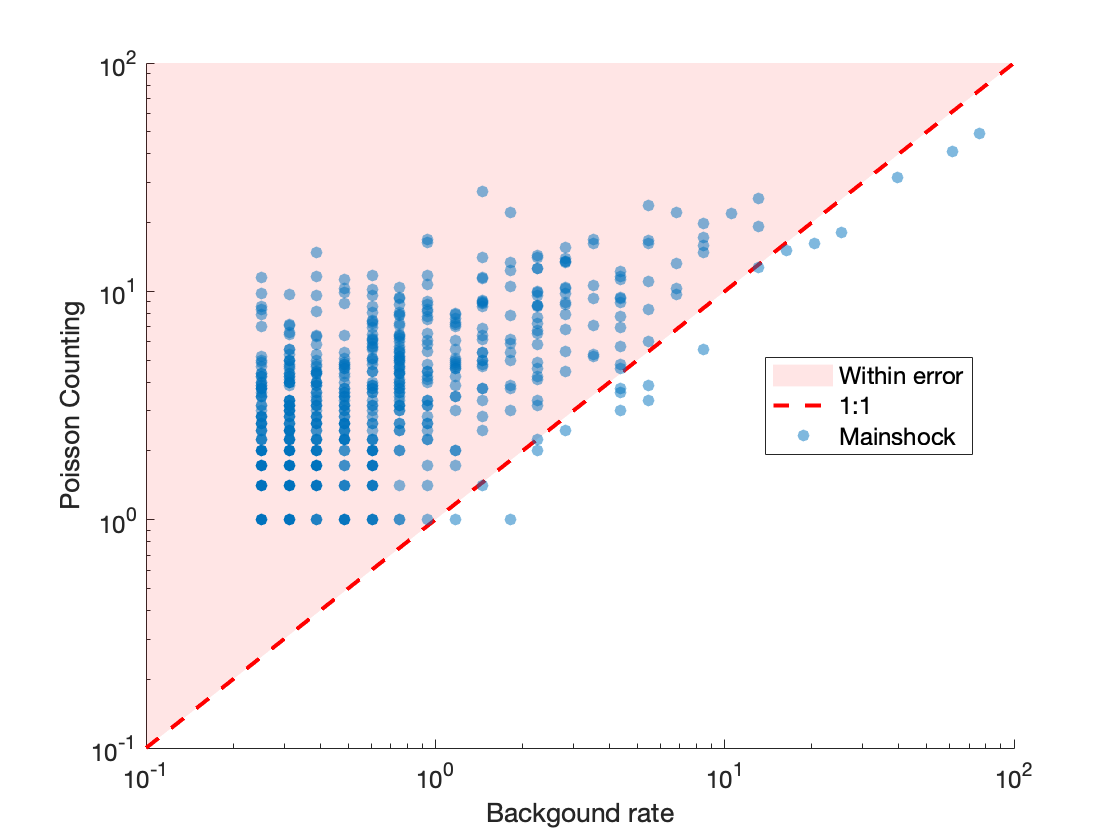
\includegraphics[width=\linewidth]{figures/does_back_matter.png}
\caption{Comparison of the apparent background seismicity to one standard deviation of a Poisson counting error. Dashed line indicates a one-to-one relationship. 97\% of events fall in the upper half of the plot highlighted in red indicating that they are within the error of the aftershock count.}
\label{fig:error_comparasion}
\end{figure}

%%%%%%%%%%%%%%%%%%%%%%%%%%%%%%%%%%%%%%%%%%%%%%%%%%%%%%  
    
\section{Relative productivity as a function of miscellaneous parameters}\label{sec:relative}

Figure \ref{fig:misc} presents how the relative productivity changes as a function of each variable we tested for in this study. 

\begin{figure}[H]
\centering
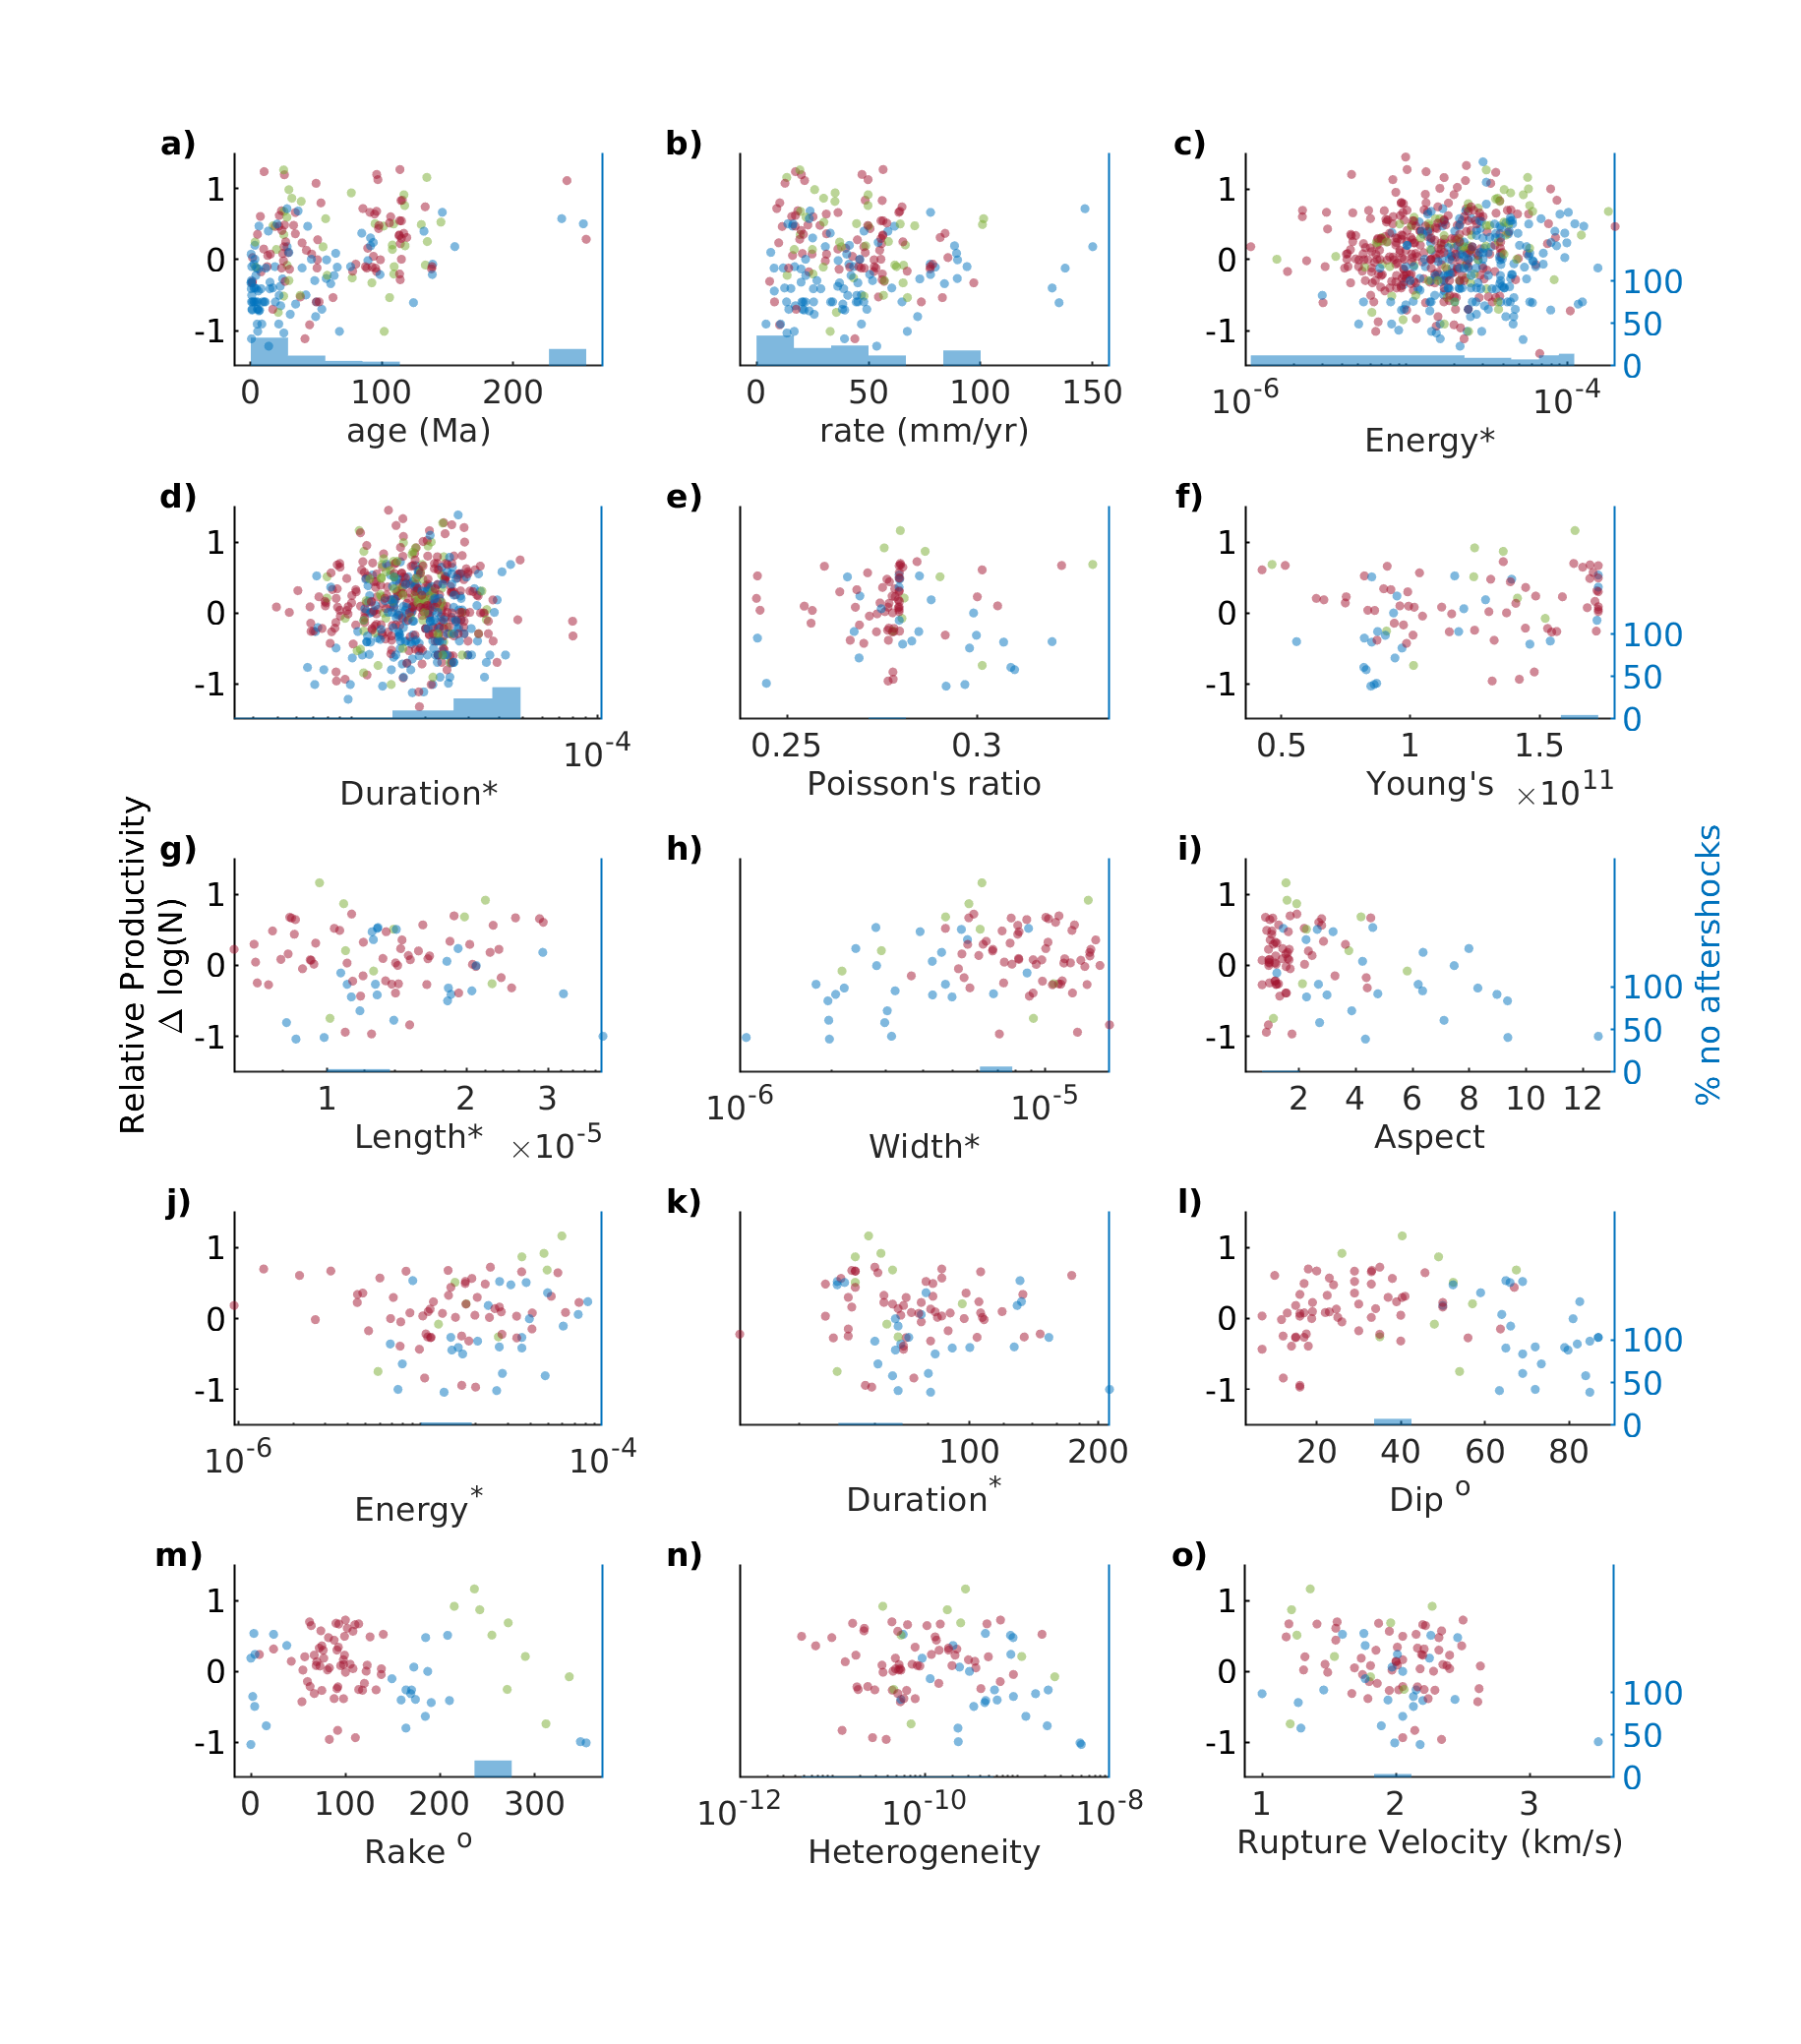
\includegraphics{figures/misc.png}
\caption{Miscellaneous setting and source attributes as a function of relative productivity ($N^*$). Source attributes that scale with magnitude are normalized (norm.) to eliminate any such dependence. Note that for the normalized rupture durations and the normalized radiated energy, we show their relationship to relative productivity for both the \citet{Convers2011GlobalMid2010} and \citet{Hayes2017} estimates. Mainshocks are color-coded by focal mechanism (strike-slip: blue, normal: green, and reverse: red). Note that a linear relationship has its limitations for more non-linear relationships (e.g. dip and rake).}
\label{fig:misc}
\end{figure}   

\section{Additional Supporting Information (Files uploaded separately)}\label{sec:additional}
\subsection{Trained SVM model}\label{sec:trained}
We provide as a separate file, \textit{train\_SVM.m}, the function used to train our SVM mode using leave-one-out cross-validation. The function includes hyperparamaters used for our analysis. Given 1) a 2-D array of predictors where rows represent individual earthquakes and columns represent predictors (in our case dip, normalized area and plate age); and 2) a response vector (in our case the relative productivity), the function returns the predictions, \textit{validationPredictions}, the root means squared error, \textit{validationRMSE}, and the trained model, \textit{regressionSVM}.

\subsection{Catalogued Source Parameters}\label{sec:source}

We provide separately a table (Table S1), \textit{FSPcat.csv}, for all the source attributes we consider. The table includes earthquake date (in \textit{matlab} \textit{datenum} format), latitude, longitude, depth (km), moment magnitude, moment (Nm), dip, rake, rupture velocity (km/s), rupture duration (s), Young's modulus (Pa), and Poisson's ratio as reported by \citet{Hayes2017}. We also include the focal mechanism, width (km), length (km), aspect ratio (length over width), slip heterogeneity and stress drop (MPa) that we derived.

\subsection{Alternative clustering method code}\label{sec:aftershock}
The full description of the alternative aftershock detection routine is  available in a Python Jupyter Notebook at the following GitHub page: https://github.com/tgoebel/clustering-analysis. In addition, this repository contains all the functions and utilities used in the process in addition to the earthquake catalog used in this study. 


\bibliography{references.bib}

\end{document}